%%%%%%%%%%%%%%%%%%%%%%%%%%%%%%%%%%%%%%%%%
% The Legrand Orange Book
% LaTeX Template
% Version 2.1 (14/11/15)
%
% This template has been downloaded from:
% http://www.LaTeXTemplates.com
%
% Mathias Legrand (legrand.mathias@gmail.com) with modifications by:
% Vel (vel@latextemplates.com)
%
% License:
% CC BY-NC-SA 3.0 (http://creativecommons.org/licenses/by-nc-sa/3.0/)
%
% Compiling this template:
% This template uses biber for its bibliography and makeindex for its index.
% When you first open the template, compile it from the command line with the 
% commands below to make sure your LaTeX distribution is configured correctly:
%
% 1) pdflatex main
% 2) makeindex main.idx -s StyleInd.ist
% 3) biber main
% 4) pdflatex main x 2
%
% After this, when you wish to update the bibliography/index use the appropriate
% command above and make sure to compile with pdflatex several times 
% afterwards to propagate your changes to the document.
%
% This template also uses a number of packages which may need to be
% updated to the newest versions for the template to compile. It is strongly
% recommended you update your LaTeX distribution if you have any
% compilation errors.
%
% Important note:
% Chapter heading images should have a 2:1 width:height ratio,
% e.g. 920px width and 460px height.
%
%%%%%%%%%%%%%%%%%%%%%%%%%%%%%%%%%%%%%%%%%

%----------------------------------------------------------------------------------------
%	PACKAGES AND OTHER DOCUMENT CONFIGURATIONS
%----------------------------------------------------------------------------------------

%\documentclass[11pt,fleqn]{book} % Default font size and left-justified equations

\documentclass[11pt,a4paper]{book} % Default font size and left-justified equations

%----------------------------------------------------------------------------------------

%%%%%%%%%%%%%%%%%%%%%%%%%%%%%%%%%%%%%%%%%
% The Legrand Orange Book
% Structural Definitions File
% Version 2.0 (9/2/15)
%
% Original author:
% Mathias Legrand (legrand.mathias@gmail.com) with modifications by:
% Vel (vel@latextemplates.com)
% 
% This file has been downloaded from:
% http://www.LaTeXTemplates.com
%
% License:
% CC BY-NC-SA 3.0 (http://creativecommons.org/licenses/by-nc-sa/3.0/)
%
%%%%%%%%%%%%%%%%%%%%%%%%%%%%%%%%%%%%%%%%%

%----------------------------------------------------------------------------------------
%	VARIOUS REQUIRED PACKAGES AND CONFIGURATIONS
%----------------------------------------------------------------------------------------

\usepackage[top=3cm,bottom=3cm,left=3cm,right=3cm,headsep=10pt,a4paper]{geometry} % Page margins

\usepackage{graphicx} % Required for including pictures
\graphicspath{{Pictures/}} % Specifies the directory where pictures are stored

\usepackage{lipsum} % Inserts dummy text

\usepackage{tikz} % Required for drawing custom shapes

\usepackage[english]{babel} % English language/hyphenation

\usepackage{enumitem} % Customize lists
\setlist{nolistsep} % Reduce spacing between bullet points and numbered lists

\usepackage{booktabs} % Required for nicer horizontal rules in tables

\usepackage{xcolor} % Required for specifying colors by name
%\definecolor{ocre}{RGB}{243,102,25} % Define the orange color used for highlighting throughout the book
\definecolor{ocre}{RGB}{0,102,25} % Define the orange color used for highlighting throughout the book

\usepackage{pdfpages}
\usepackage{multicol} % use of multiple columns
\columnsep=8mm
%\usepackage[print]{booklet}

%----------------------------------------------------------------------------------------
%	FONTS
%----------------------------------------------------------------------------------------

\usepackage{avant} % Use the Avantgarde font for headings
%\usepackage{times} % Use the Times font for headings
\usepackage{mathptmx} % Use the Adobe Times Roman as the default text font together with math symbols from the Sym­bol, Chancery and Com­puter Modern fonts

\usepackage{microtype} % Slightly tweak font spacing for aesthetics
\usepackage[utf8]{inputenc} % Required for including letters with accents
\usepackage[T1]{fontenc} % Use 8-bit encoding that has 256 glyphs

\setlength{\parskip}{2mm}
\setlength{\parindent}{0mm} % Default is 15pt.

%----------------------------------------------------------------------------------------
%	BIBLIOGRAPHY AND INDEX
%----------------------------------------------------------------------------------------

\usepackage[style=alphabetic,citestyle=numeric,sorting=nyt,sortcites=true,autopunct=true,babel=hyphen,hyperref=true,abbreviate=false,backref=true,backend=biber]{biblatex}
\addbibresource{bibliography.bib} % BibTeX bibliography file
\defbibheading{bibempty}{}

\usepackage{calc} % For simpler calculation - used for spacing the index letter headings correctly
\usepackage{makeidx} % Required to make an index
\makeindex % Tells LaTeX to create the files required for indexing

%----------------------------------------------------------------------------------------
%	MAIN TABLE OF CONTENTS
%----------------------------------------------------------------------------------------

\usepackage{titletoc} % Required for manipulating the table of contents

\contentsmargin{0cm} % Removes the default margin

% Part text styling
\titlecontents{part}[0cm]
{\addvspace{20pt}\centering\large\bfseries}
{}
{}
{}

% Chapter text styling
\titlecontents{chapter}[1.25cm] % Indentation
{\addvspace{12pt}\large\sffamily\bfseries} % Spacing and font options for chapters
{\color{ocre!60}\contentslabel[\Large\thecontentslabel]{1.25cm}\color{ocre}} % Chapter number
{\color{ocre}}  
{\color{ocre!60}\normalsize\;\titlerule*[.5pc]{.}\;\thecontentspage} % Page number

% Section text styling
\titlecontents{section}[1.25cm] % Indentation
{\addvspace{3pt}\sffamily\bfseries} % Spacing and font options for sections
{\contentslabel[\thecontentslabel]{1.25cm}} % Section number
{}
{\hfill\color{black}\thecontentspage} % Page number
[]

% Subsection text styling
\titlecontents{subsection}[1.25cm] % Indentation
{\addvspace{1pt}\sffamily\small} % Spacing and font options for subsections
{\contentslabel[\thecontentslabel]{1.25cm}} % Subsection number
{}
{\ \titlerule*[.5pc]{.}\;\thecontentspage} % Page number
[]

% List of figures
\titlecontents{figure}[0em]
{\addvspace{-5pt}\sffamily}
{\thecontentslabel\hspace*{1em}}
{}
{\ \titlerule*[.5pc]{.}\;\thecontentspage}
[]

% List of tables
\titlecontents{table}[0em]
{\addvspace{-5pt}\sffamily}
{\thecontentslabel\hspace*{1em}}
{}
{\ \titlerule*[.5pc]{.}\;\thecontentspage}
[]

%----------------------------------------------------------------------------------------
%	MINI TABLE OF CONTENTS IN PART HEADS
%----------------------------------------------------------------------------------------

% Chapter text styling
\titlecontents{lchapter}[-8em] % Indenting
{\addvspace{15pt}\large\sffamily\bfseries} % Spacing and font options for chapters
{\color{ocre}\contentslabel[\Large\thecontentslabel]{1.25cm}\color{ocre}} % Chapter number
{}  
{\color{ocre}\normalsize\sffamily\bfseries\;\titlerule*[.5pc]{.}\;\thecontentspage} % Page number

% Section text styling
\titlecontents{lsection}[-8em] % Indenting
{\addvspace{6pt}\sffamily\small} % Spacing and font options for sections
{\contentslabel[\thecontentslabel]{1.25cm}} % Section number
{}
{}

% Subsection text styling
\titlecontents{lsubsection}[.5em] % Indentation
{\normalfont\footnotesize\sffamily} % Font settings
{}
{}
{}

%----------------------------------------------------------------------------------------
%	PAGE HEADERS
%----------------------------------------------------------------------------------------

\usepackage{fancyhdr} % Required for header and footer configuration

\pagestyle{fancy}
\renewcommand{\chaptermark}[1]{\markboth{\sffamily\normalsize\bfseries\chaptername\ \thechapter.\ #1}{}} % Chapter text font settings
\renewcommand{\sectionmark}[1]{\markright{\sffamily\normalsize\thesection\hspace{5pt}#1}{}} % Section text font settings
\fancyhf{} \fancyhead[LE,RO]{\sffamily\normalsize\thepage} % Font setting for the page number in the header
\fancyhead[LO]{\leftmark} % Print the nearest section name on the left side of odd pages
\fancyhead[RE]{\leftmark} % Print the current chapter name on the right side of even pages
\renewcommand{\headrulewidth}{0.5pt} % Width of the rule under the header
\addtolength{\headheight}{2.5pt} % Increase the spacing around the header slightly
\renewcommand{\footrulewidth}{0pt} % Removes the rule in the footer
\fancypagestyle{plain}{\fancyhead{}\renewcommand{\headrulewidth}{0pt}} % Style for when a plain pagestyle is specified

% Removes the header from odd empty pages at the end of chapters
\makeatletter
\renewcommand{\cleardoublepage}{
\clearpage\ifodd\c@page\else
\hbox{}
\vspace*{\fill}
\thispagestyle{empty}
\newpage
\fi}

%----------------------------------------------------------------------------------------
%	THEOREM STYLES
%----------------------------------------------------------------------------------------

\usepackage{amsmath,amsfonts,amssymb,amsthm} % For math equations, theorems, symbols, etc

\newcommand{\intoo}[2]{\mathopen{]}#1\,;#2\mathclose{[}}
\newcommand{\ud}{\mathop{\mathrm{{}d}}\mathopen{}}
\newcommand{\intff}[2]{\mathopen{[}#1\,;#2\mathclose{]}}
\newtheorem{notation}{Notation}[chapter]

% Boxed/framed environments
\newtheoremstyle{ocrenumbox}% % Theorem style name
{0pt}% Space above
{0pt}% Space below
{\normalfont}% % Body font
{}% Indent amount
{\small\bf\sffamily\color{ocre}}% % Theorem head font
{\;}% Punctuation after theorem head
{0.25em}% Space after theorem head
{\small\sffamily\color{ocre}\thmname{#1}\nobreakspace\thmnumber{\@ifnotempty{#1}{}\@upn{#2}}% Theorem text (e.g. Theorem 2.1)
\thmnote{\nobreakspace\the\thm@notefont\sffamily\bfseries\color{black}---\nobreakspace#3.}} % Optional theorem note
\renewcommand{\qedsymbol}{$\blacksquare$}% Optional qed square

\newtheoremstyle{blacknumex}% Theorem style name
{5pt}% Space above
{5pt}% Space below
{\normalfont}% Body font
{} % Indent amount
{\small\bf\sffamily}% Theorem head font
{\;}% Punctuation after theorem head
{0.25em}% Space after theorem head
{\small\sffamily{\tiny\ensuremath{\blacksquare}}\nobreakspace\thmname{#1}\nobreakspace\thmnumber{\@ifnotempty{#1}{}\@upn{#2}}% Theorem text (e.g. Theorem 2.1)
\thmnote{\nobreakspace\the\thm@notefont\sffamily\bfseries---\nobreakspace#3.}}% Optional theorem note

\newtheoremstyle{blacknumbox} % Theorem style name
{0pt}% Space above
{0pt}% Space below
{\normalfont}% Body font
{}% Indent amount
{\small\bf\sffamily}% Theorem head font
{\;}% Punctuation after theorem head
{0.25em}% Space after theorem head
{\small\sffamily\thmname{#1}\nobreakspace\thmnumber{\@ifnotempty{#1}{}\@upn{#2}}% Theorem text (e.g. Theorem 2.1)
\thmnote{\nobreakspace\the\thm@notefont\sffamily\bfseries---\nobreakspace#3.}}% Optional theorem note

% Non-boxed/non-framed environments
\newtheoremstyle{ocrenum}% % Theorem style name
{5pt}% Space above
{5pt}% Space below
{\normalfont}% % Body font
{}% Indent amount
{\small\bf\sffamily\color{ocre}}% % Theorem head font
{\;}% Punctuation after theorem head
{0.25em}% Space after theorem head
{\small\sffamily\color{ocre}\thmname{#1}\nobreakspace\thmnumber{\@ifnotempty{#1}{}\@upn{#2}}% Theorem text (e.g. Theorem 2.1)
\thmnote{\nobreakspace\the\thm@notefont\sffamily\bfseries\color{black}---\nobreakspace#3.}} % Optional theorem note
\renewcommand{\qedsymbol}{$\blacksquare$}% Optional qed square
\makeatother

% Defines the theorem text style for each type of theorem to one of the three styles above
\newcounter{dummy} 
\numberwithin{dummy}{section}
\theoremstyle{ocrenumbox}
\newtheorem{theoremeT}[dummy]{Theorem}
\newtheorem{problem}{Problem}[chapter]
\newtheorem{exerciseT}{Exercise}[chapter]
\theoremstyle{blacknumex}
\newtheorem{exampleT}{Example}[chapter]
\theoremstyle{blacknumbox}
\newtheorem{vocabulary}{Vocabulary}[chapter]
\newtheorem{definitionT}{Definition}[section]
\newtheorem{corollaryT}[dummy]{Corollary}
\theoremstyle{ocrenum}
\newtheorem{proposition}[dummy]{Proposition}

%----------------------------------------------------------------------------------------
%	DEFINITION OF COLORED BOXES
%----------------------------------------------------------------------------------------

\RequirePackage[framemethod=default]{mdframed} % Required for creating the theorem, definition, exercise and corollary boxes

% Theorem box
\newmdenv[skipabove=7pt,
skipbelow=7pt,
backgroundcolor=black!5,
linecolor=ocre,
innerleftmargin=5pt,
innerrightmargin=5pt,
innertopmargin=5pt,
leftmargin=0cm,
rightmargin=0cm,
innerbottommargin=5pt]{tBox}

% Exercise box	  
\newmdenv[skipabove=7pt,
skipbelow=7pt,
rightline=false,
leftline=true,
topline=false,
bottomline=false,
backgroundcolor=ocre!10,
linecolor=ocre,
innerleftmargin=5pt,
innerrightmargin=5pt,
innertopmargin=5pt,
innerbottommargin=5pt,
leftmargin=0cm,
rightmargin=0cm,
linewidth=4pt]{eBox}	

% Definition box
\newmdenv[skipabove=7pt,
skipbelow=7pt,
rightline=false,
leftline=true,
topline=false,
bottomline=false,
linecolor=ocre,
innerleftmargin=5pt,
innerrightmargin=5pt,
innertopmargin=0pt,
leftmargin=0cm,
rightmargin=0cm,
linewidth=4pt,
innerbottommargin=0pt]{dBox}	

% Corollary box
\newmdenv[skipabove=7pt,
skipbelow=7pt,
rightline=false,
leftline=true,
topline=false,
bottomline=false,
linecolor=gray,
backgroundcolor=black!5,
innerleftmargin=5pt,
innerrightmargin=5pt,
innertopmargin=5pt,
leftmargin=0cm,
rightmargin=0cm,
linewidth=4pt,
innerbottommargin=5pt]{cBox}

% Creates an environment for each type of theorem and assigns it a theorem text style from the "Theorem Styles" section above and a colored box from above
\newenvironment{theorem}{\begin{tBox}\begin{theoremeT}}{\end{theoremeT}\end{tBox}}
\newenvironment{exercise}{\begin{eBox}\begin{exerciseT}}{\hfill{\color{ocre}\tiny\ensuremath{\blacksquare}}\end{exerciseT}\end{eBox}}				  
\newenvironment{definition}{\begin{dBox}\begin{definitionT}}{\end{definitionT}\end{dBox}}	
\newenvironment{example}{\begin{exampleT}}{\hfill{\tiny\ensuremath{\blacksquare}}\end{exampleT}}		
\newenvironment{corollary}{\begin{cBox}\begin{corollaryT}}{\end{corollaryT}\end{cBox}}	

%----------------------------------------------------------------------------------------
%	REMARK ENVIRONMENT
%----------------------------------------------------------------------------------------

\newenvironment{remark}{\par\vspace{10pt}\small % Vertical white space above the remark and smaller font size
\begin{list}{}{
\leftmargin=35pt % Indentation on the left
\rightmargin=25pt}\item\ignorespaces % Indentation on the right
\makebox[-2.5pt]{\begin{tikzpicture}[overlay]
\node[draw=ocre!60,line width=1pt,circle,fill=ocre!25,font=\sffamily\bfseries,inner sep=2pt,outer sep=0pt] at (-15pt,0pt){\textcolor{ocre}{R}};\end{tikzpicture}} % Orange R in a circle
\advance\baselineskip -1pt}{\end{list}\vskip5pt} % Tighter line spacing and white space after remark

%----------------------------------------------------------------------------------------
%	SECTION NUMBERING IN THE MARGIN
%----------------------------------------------------------------------------------------

\makeatletter
\renewcommand{\@seccntformat}[1]{\llap{\textcolor{ocre}{\csname the#1\endcsname}\hspace{1em}}}                    
\renewcommand{\section}{\@startsection{section}{1}{\z@}
{-4ex \@plus -1ex \@minus -.4ex}
{1ex \@plus.2ex }
{\normalfont\large\sffamily\bfseries}}
\renewcommand{\subsection}{\@startsection {subsection}{2}{\z@}
{-3ex \@plus -0.1ex \@minus -.4ex}
{0.5ex \@plus.2ex }
{\normalfont\sffamily\bfseries}}
\renewcommand{\subsubsection}{\@startsection {subsubsection}{3}{\z@}
{-2ex \@plus -0.1ex \@minus -.2ex}
{.2ex \@plus.2ex }
{\normalfont\small\sffamily\bfseries}}                        
\renewcommand\paragraph{\@startsection{paragraph}{4}{\z@}
{-2ex \@plus-.2ex \@minus .2ex}
{.1ex}
{\normalfont\small\sffamily\bfseries}}

%----------------------------------------------------------------------------------------
%	PART HEADINGS
%----------------------------------------------------------------------------------------

% numbered part in the table of contents
\newcommand{\@mypartnumtocformat}[2]{%
\setlength\fboxsep{0pt}%
\noindent\colorbox{ocre!20}{\strut\parbox[c][.7cm]{\ecart}{\color{ocre!70}\Large\sffamily\bfseries\centering#1}}\hskip\esp\colorbox{ocre!40}{\strut\parbox[c][.7cm]{\linewidth-\ecart-\esp}{\Large\sffamily\centering#2}}}%
%%%%%%%%%%%%%%%%%%%%%%%%%%%%%%%%%%
% unnumbered part in the table of contents
\newcommand{\@myparttocformat}[1]{%
\setlength\fboxsep{0pt}%
\noindent\colorbox{ocre!40}{\strut\parbox[c][.7cm]{\linewidth}{\Large\sffamily\centering#1}}}%
%%%%%%%%%%%%%%%%%%%%%%%%%%%%%%%%%%
\newlength\esp
\setlength\esp{4pt}
\newlength\ecart
\setlength\ecart{1.2cm-\esp}
\newcommand{\thepartimage}{}%
\newcommand{\partimage}[1]{\renewcommand{\thepartimage}{#1}}%
\def\@part[#1]#2{%
\ifnum \c@secnumdepth >-2\relax%
\refstepcounter{part}%
\addcontentsline{toc}{part}{\texorpdfstring{\protect\@mypartnumtocformat{\thepart}{#1}}{\partname~\thepart\ ---\ #1}}
\else%
\addcontentsline{toc}{part}{\texorpdfstring{\protect\@myparttocformat{#1}}{#1}}%
\fi%
\startcontents%
\markboth{}{}%
{\thispagestyle{empty}%
\begin{tikzpicture}[remember picture,overlay]%
\node at (current page.north west){\begin{tikzpicture}[remember picture,overlay]%	
\fill[ocre!20](0cm,0cm) rectangle (\paperwidth,-\paperheight);
\node[anchor=north] at (4cm,-3.25cm){\color{ocre!40}\fontsize{220}{100}\sffamily\bfseries\@Roman\c@part}; 
\node[anchor=south east] at (\paperwidth-1cm,-\paperheight+1cm){\parbox[t][][t]{8.5cm}{
\printcontents{l}{0}{\setcounter{tocdepth}{1}}%
}};
\node[anchor=north east] at (\paperwidth-1.5cm,-3.25cm){\parbox[t][][t]{15cm}{\strut\raggedleft\color{white}\fontsize{30}{30}\sffamily\bfseries#2}};
\end{tikzpicture}};
\end{tikzpicture}}%
\@endpart}
\def\@spart#1{%
\startcontents%
\phantomsection
{\thispagestyle{empty}%
\begin{tikzpicture}[remember picture,overlay]%
\node at (current page.north west){\begin{tikzpicture}[remember picture,overlay]%	
\fill[ocre!20](0cm,0cm) rectangle (\paperwidth,-\paperheight);
\node[anchor=north east] at (\paperwidth-1.5cm,-3.25cm){\parbox[t][][t]{15cm}{\strut\raggedleft\color{white}\fontsize{30}{30}\sffamily\bfseries#1}};
\end{tikzpicture}};
\end{tikzpicture}}
\addcontentsline{toc}{part}{\texorpdfstring{%
\setlength\fboxsep{0pt}%
\noindent\protect\colorbox{ocre!40}{\strut\protect\parbox[c][.7cm]{\linewidth}{\Large\sffamily\protect\centering #1\quad\mbox{}}}}{#1}}%
\@endpart}
\def\@endpart{\vfil\newpage
\if@twoside
\if@openright
\null
\thispagestyle{empty}%
\newpage
\fi
\fi
\if@tempswa
\twocolumn
\fi}

%----------------------------------------------------------------------------------------
%	CHAPTER HEADINGS
%----------------------------------------------------------------------------------------

\newcommand{\thechapterimage}{}%
\newcommand{\chapterimage}[1]{\renewcommand{\thechapterimage}{#1}}%
\def\@makechapterhead#1{%
{\parindent \z@ \raggedright \normalfont
\ifnum \c@secnumdepth >\m@ne
\if@mainmatter
\begin{tikzpicture}[remember picture,overlay]
\node at (current page.north west)
{\begin{tikzpicture}[remember picture,overlay]
\node[anchor=north west,inner sep=0pt] at (0,0) {\includegraphics[width=\paperwidth]{\thechapterimage}};
%\draw[anchor=west] (\Gm@lmargin,-9cm) node [line width=2pt,rounded corners=15pt,draw=ocre,fill=white,fill opacity=0.5,inner sep=15pt]{\strut\makebox[22cm]{}};
\draw[anchor=west] (\Gm@lmargin,-7cm) node [fill=white,fill opacity=0.5,inner sep=15pt]{\strut\makebox[22cm]{}};
\draw[anchor=west] (\Gm@lmargin+.3cm,-7cm) node {\huge\sffamily\bfseries\color{black}\thechapter. #1\strut};
\end{tikzpicture}};
\end{tikzpicture}
\else
\begin{tikzpicture}[remember picture,overlay]
\node at (current page.north west)
{\begin{tikzpicture}[remember picture,overlay]
\node[anchor=north west,inner sep=0pt] at (0,0) {\includegraphics[width=\paperwidth]{\thechapterimage}};
%\draw[anchor=west] (\Gm@lmargin,-9cm) node [line width=2pt,rounded corners=15pt,draw=ocre,fill=white,fill opacity=0.5,inner sep=15pt]{\strut\makebox[22cm]{}};
\draw[anchor=west] (\Gm@lmargin,-7cm) node [fill=white,fill opacity=0.5,inner sep=15pt]{\strut\makebox[22cm]{}};
\draw[anchor=west] (\Gm@lmargin+.3cm,-7cm) node {\huge\sffamily\bfseries\color{black}#1\strut};
\end{tikzpicture}};
\end{tikzpicture}
\fi\fi\par\vspace*{270\p@}}}

%-------------------------------------------

\def\@makeschapterhead#1{%
\begin{tikzpicture}[remember picture,overlay]
\node at (current page.north west)
{\begin{tikzpicture}[remember picture,overlay]
\node[anchor=north west,inner sep=0pt] at (0,0) {\includegraphics[width=\paperwidth]{\thechapterimage}};
%\draw[anchor=west] (\Gm@lmargin,-9cm) node [line width=2pt,rounded corners=15pt,draw=ocre,fill=white,fill opacity=0.5,inner sep=15pt]{\strut\makebox[22cm]{}};
\draw[anchor=west] (\Gm@lmargin,-7cm) node [draw=ocre,fill=white,fill opacity=0.5,inner sep=15pt]{\strut\makebox[22cm]{}};
\draw[anchor=west] (\Gm@lmargin+.3cm,-7cm) node {\huge\sffamily\bfseries\color{black}#1\strut};
\end{tikzpicture}};
\end{tikzpicture}
\par\vspace*{270\p@}}
\makeatother

%----------------------------------------------------------------------------------------
%	HYPERLINKS IN THE DOCUMENTS
%----------------------------------------------------------------------------------------

\usepackage{hyperref}
\hypersetup{hidelinks,backref=true,pagebackref=true,hyperindex=true,colorlinks=false,breaklinks=true,urlcolor= ocre,bookmarks=true,bookmarksopen=false,pdftitle={Title},pdfauthor={Author}}
\usepackage{bookmark}
\bookmarksetup{
open,
numbered,
addtohook={%
\ifnum\bookmarkget{level}=0 % chapter
\bookmarksetup{bold}%
\fi
\ifnum\bookmarkget{level}=-1 % part
\bookmarksetup{color=ocre,bold}%
\fi
}
} % Insert the commands.tex file which contains the majority of the structure behind the template

\newcommand{\numpaperspt}{15 }
\newcommand{\numpapersen}{15 }
\newcommand{\Numpaperspt}{Quinze }
\newcommand{\Numpapersen}{Fifteen }
%\usepackage{draftwatermark}
%\SetWatermarkText{PRELIMINAR}
%\SetWatermarkScale{.7}
%\SetWatermarkColor[rgb]{red!60}

\begin{document}

%----------------------------------------------------------------------------------------
%	TITLE PAGE
%----------------------------------------------------------------------------------------

\begingroup
\thispagestyle{empty}
\begin{tikzpicture}[remember picture,overlay]
\coordinate [below=12cm] (midpoint) at (current page.north);
\node at (current page.north west)
{\begin{tikzpicture}[remember picture,overlay]
\node[anchor=north west,inner sep=0pt] at (0,0) {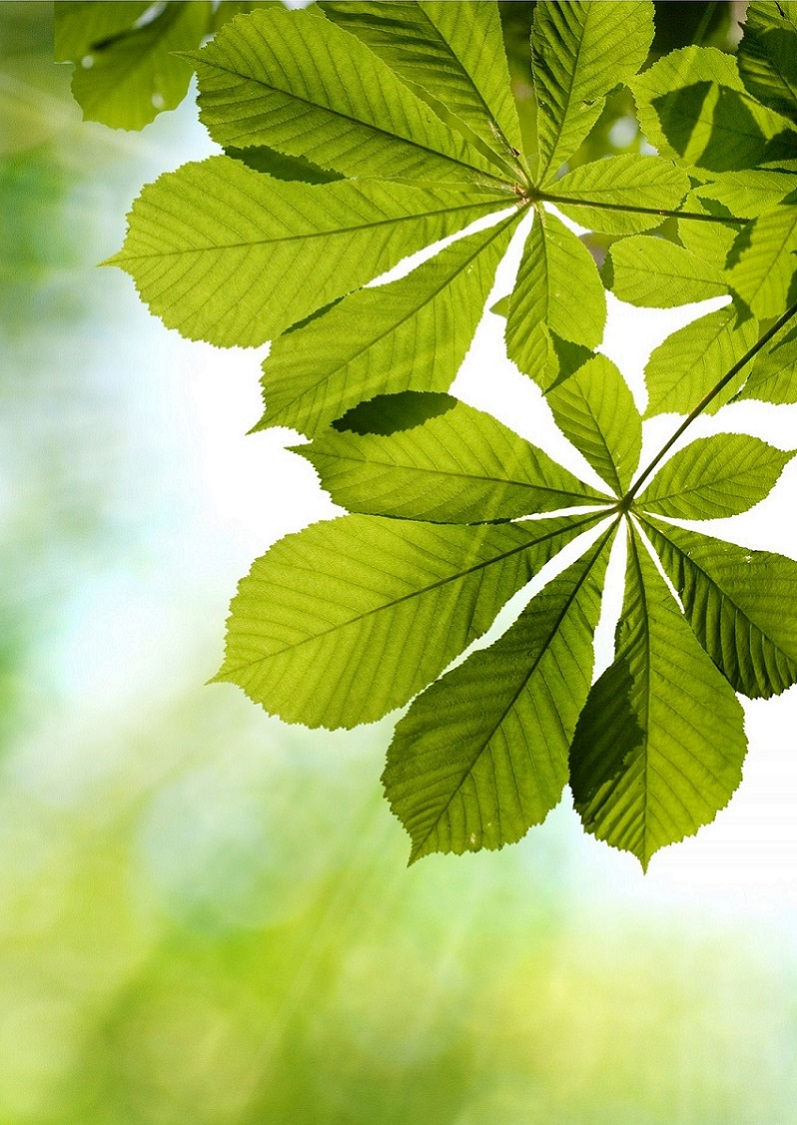
\includegraphics{leafs_04}}; % Background image
%\node[anchor=north west,inner sep=0pt] at (0,0) {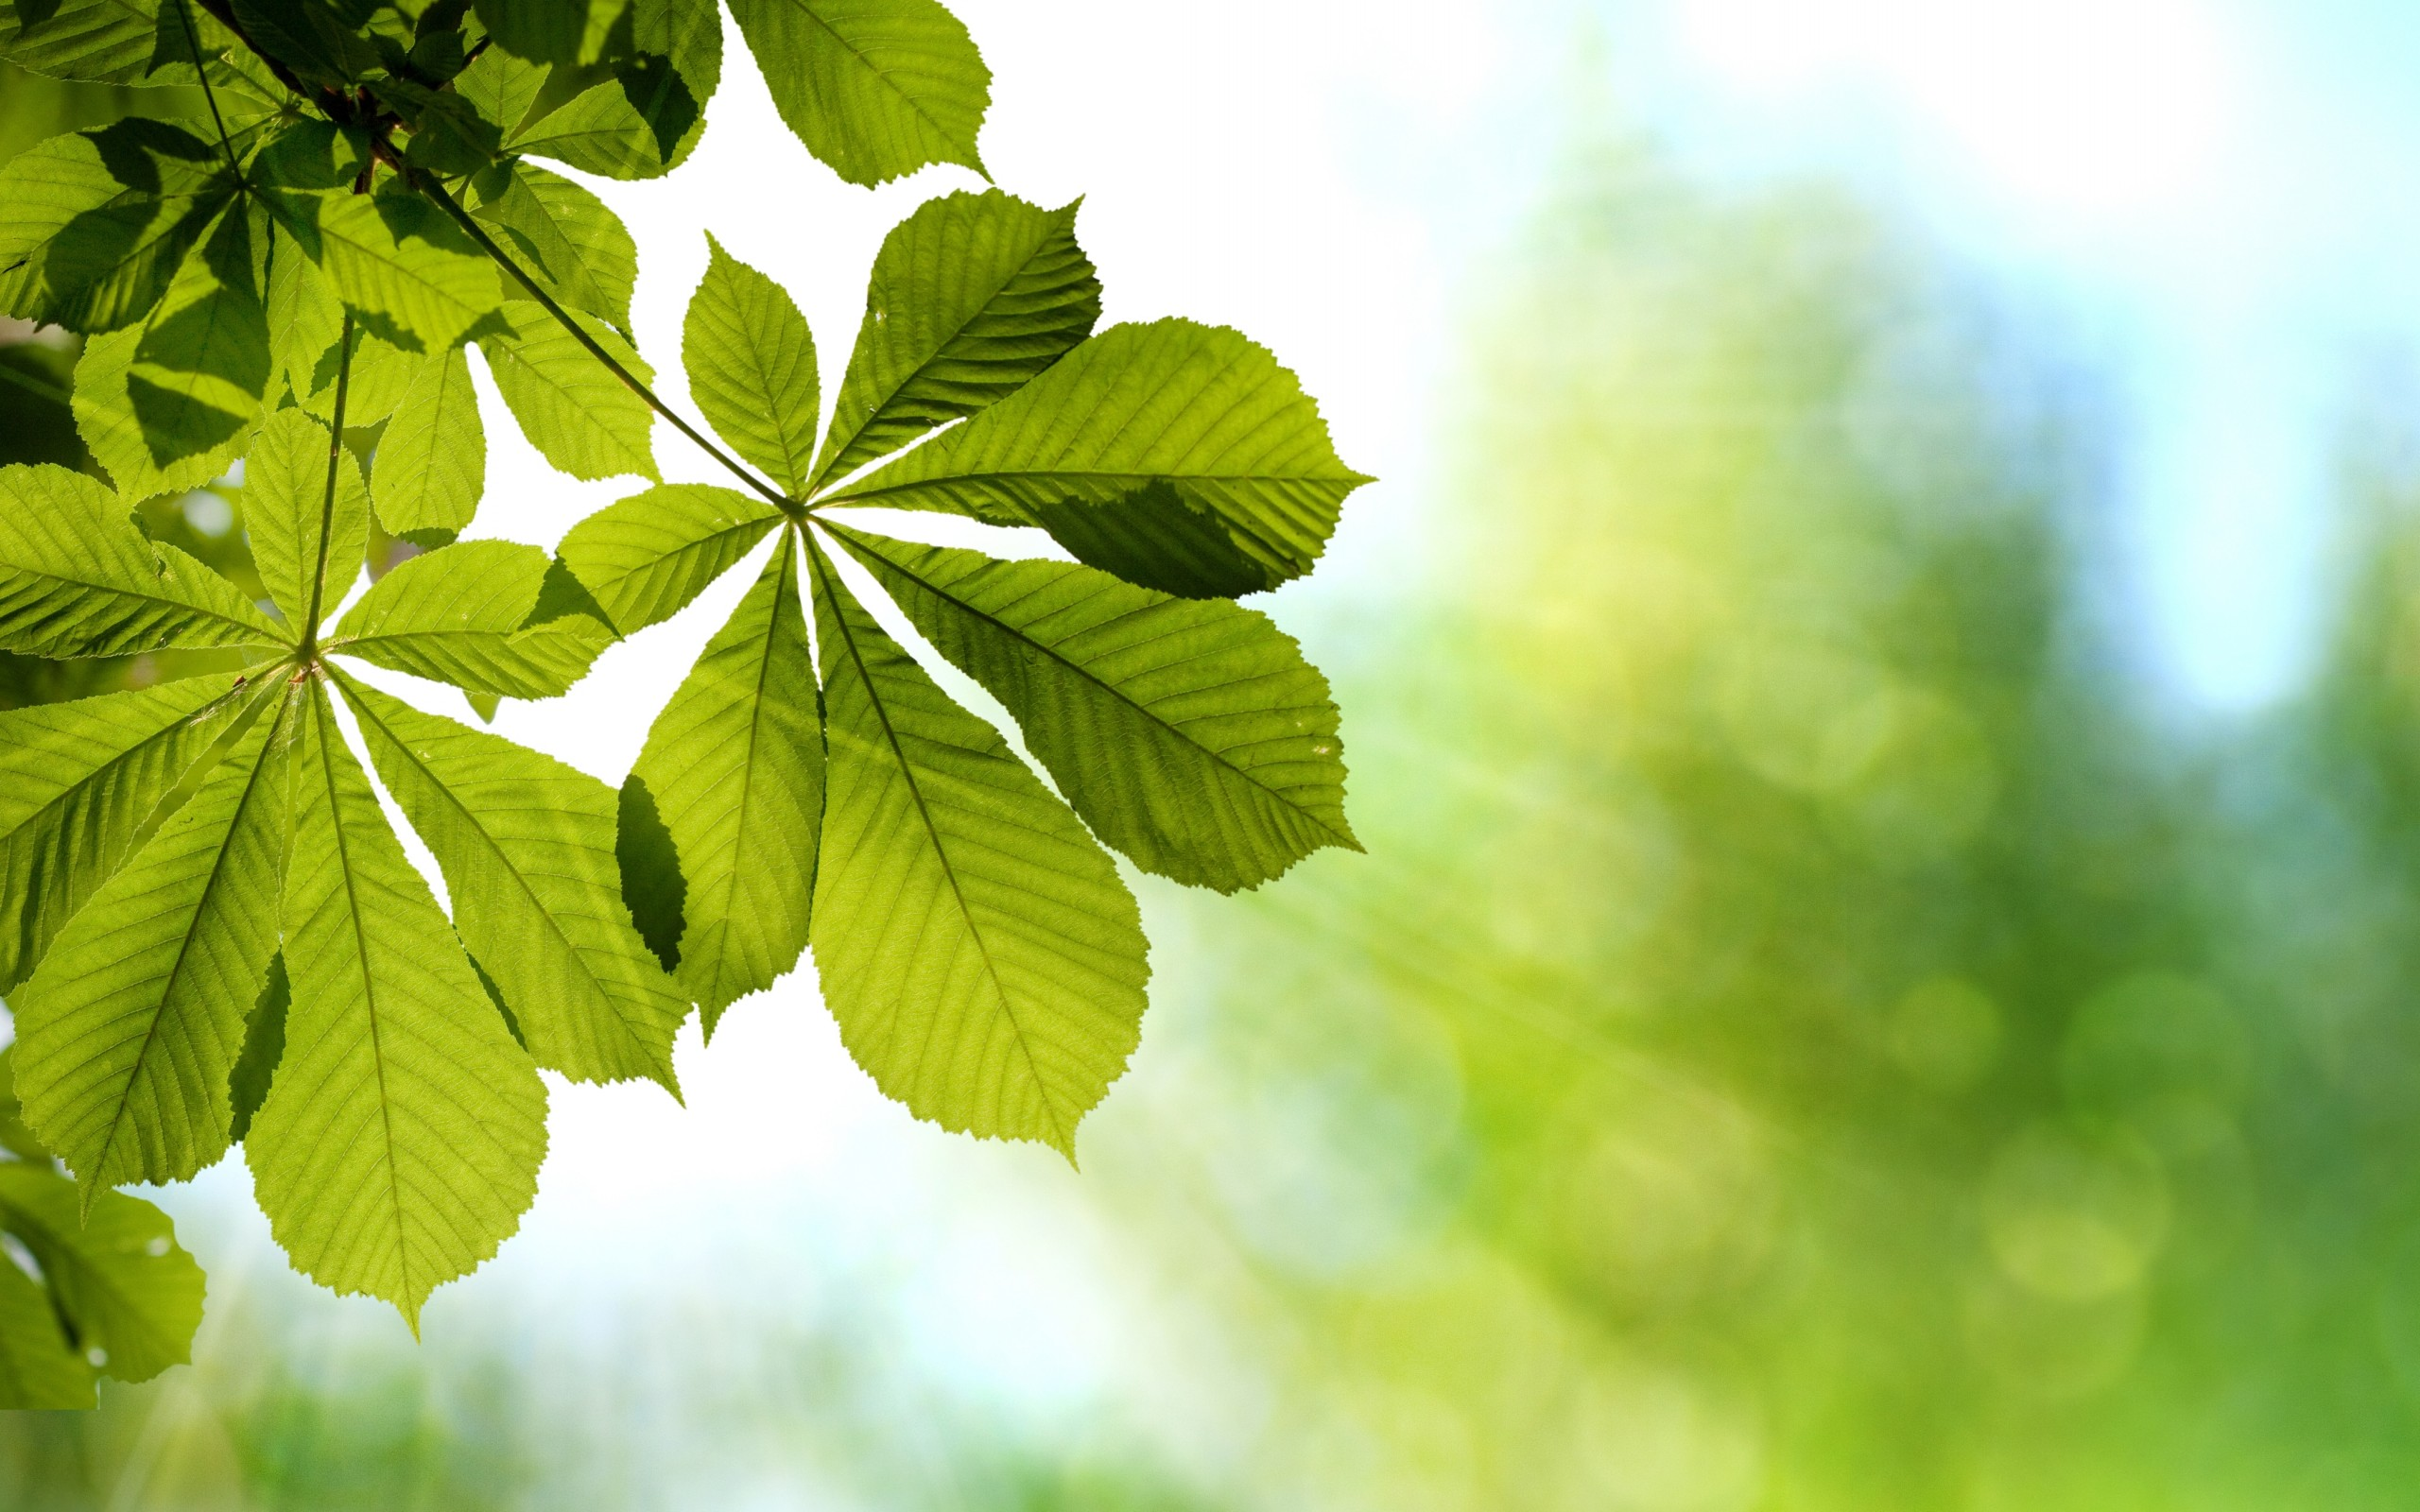
\includegraphics[scale=.5,angle=-90,origin=c]{leafs_02}}; % Background image
\draw[anchor=north] (midpoint) node [fill=ocre!30!white,fill opacity=0.6,text opacity=1,inner sep=1cm]{\Huge\centering\bfseries\sffamily\parbox[c][][t]{.9\paperwidth}{\centering SEMINÁRIOS PPG-EM / UERJ 2015\\[15pt] % Book title
{\huge PPG-EM UERJ 2015 SEMINARS}\\[20pt] % Subtitle
{\Large Programa de Pós-graduação em Engenharia Mecânica UERJ}
}}; % Author name
\end{tikzpicture}};
\end{tikzpicture}
%\vspace*{200mm}\\
%
\includegraphics[height=32mm]{Pictures/logo_uerj_PB.png}
%
\includegraphics[height=24mm]{Pictures/logo_ppg-em.png}
\vfill

\newpage
\vspace*{\fill}
\thispagestyle{empty}

\newpage
\thispagestyle{empty}
\vspace*{45mm}
\begin{center}
	
\includegraphics[height=36mm]{Pictures/logo_uerj_PB.png}\\[20mm]
	{\Huge\bfseries\sffamily SEMINÁRIOS PPG-EM / UERJ 2015\\[15pt]
	\huge PPG-EM UERJ 2015 SEMINARS\\[20pt]
	\Large Programa de Pós-graduação em Engenharia Mecânica UERJ
	}
\end{center}

%{\begin{tikzpicture}%[remember picture,overlay]
%	\node[anchor=north west,inner sep=0pt] at (0,0) %{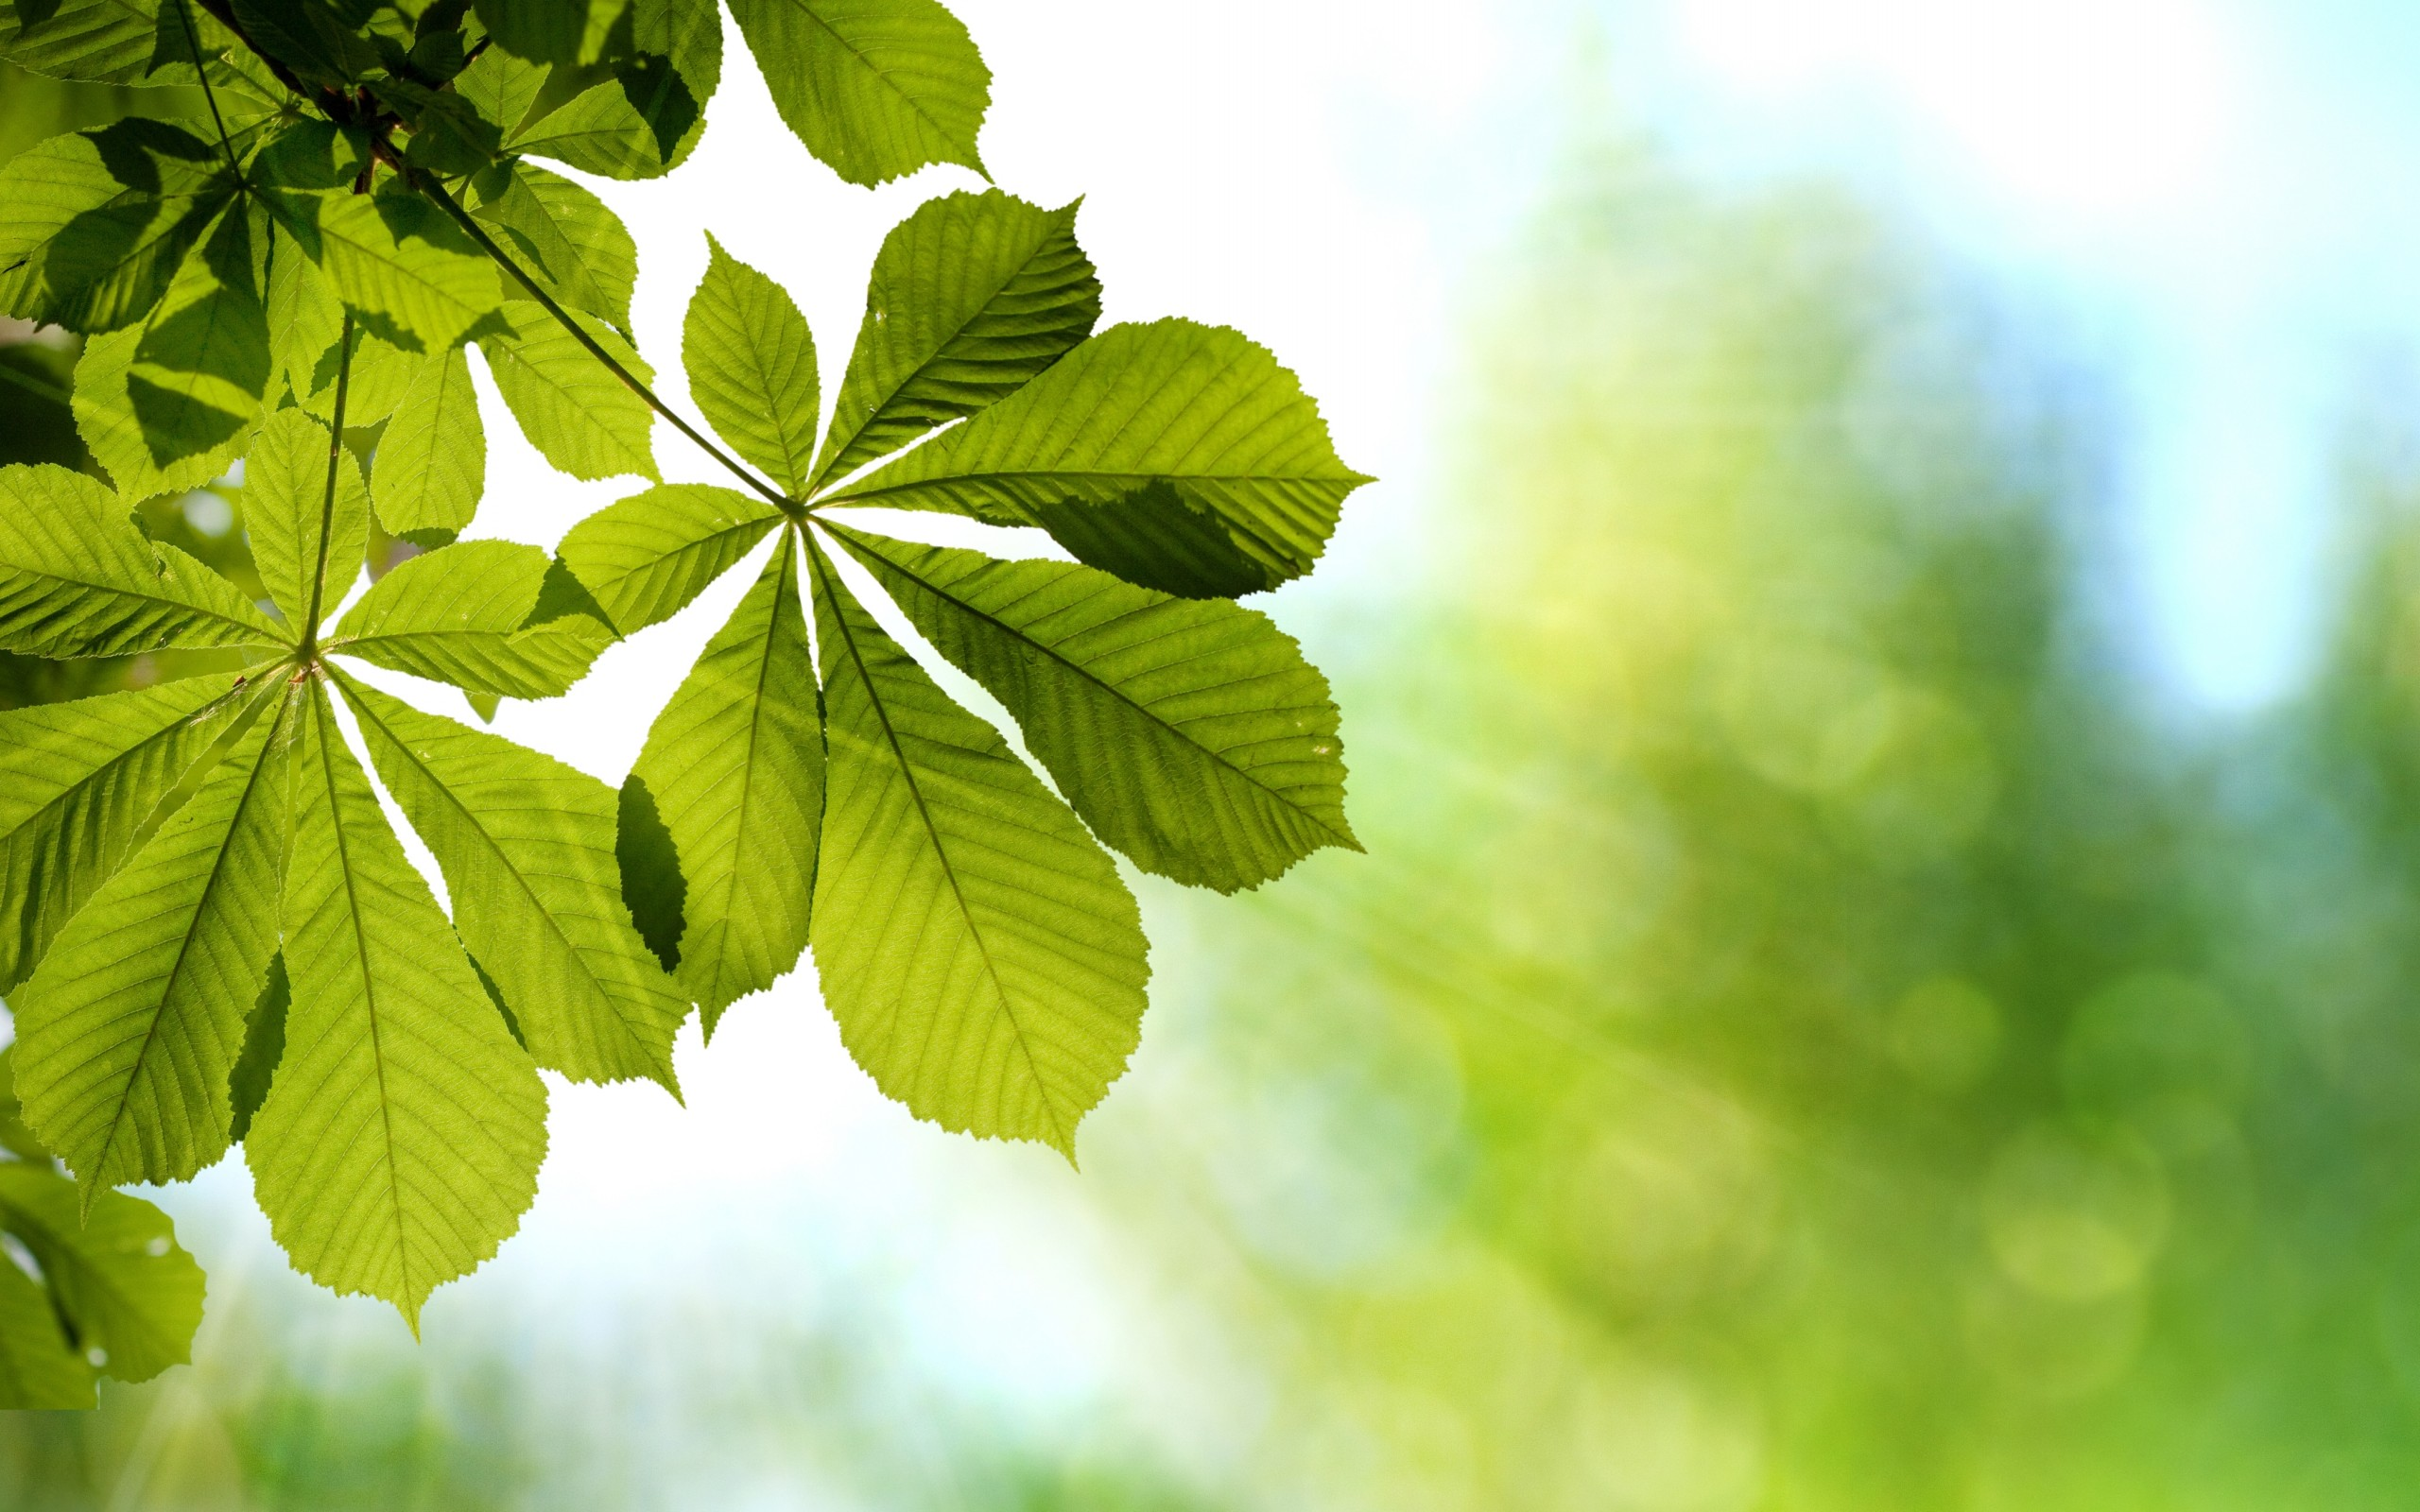
\includegraphics[scale=.5,angle=-90,origin=c]{leafs_02}}; % Background image
%	\draw[anchor=north] (midpoint) node [fill=ocre!30!white,fill opacity=0.6,text opacity=1,inner sep=1cm]
%	{\Huge\centering\bfseries\sffamily\parbox[c][][t]{\paperwidth}{\centering SEMINÁRIOS PPG-EM / UERJ 2015\\[15pt] % Book title
%	{\huge PPG-EM UERJ 2015 SEMINARS}\\[20pt] % Subtitle
%	{\Large Programa de Pós-graduação em Engenharia Mecânica UERJ}
%	}}; % Author name
%\end{tikzpicture}};
\vspace*{\fill}

\endgroup

%----------------------------------------------------------------------------------------
%	EXPEDIENTE
%----------------------------------------------------------------------------------------
\newpage
~\vfill
\thispagestyle{empty}
	\begin{center}
	\vspace*{85mm}
	{%CATALOGAÇÃO NA FONTE\\ \vspace{1.5mm}
	%UERJ\,/\,REDE SIRIUS\,/\,BIBLIOTECA CTC/B}\\
	EXPEDIENTE}\\
	\vspace{1.5mm}
	\begin{boxedminipage}{140mm}
	\begin{minipage}{5mm}
		\vspace{-80mm}
		%C837
	\end{minipage}
	\hfill
	\raisebox{8.5mm}{
	\begin{minipage}[top]{115mm}
		\vspace*{5mm}
       Programa de Pós-Graduação em Engenharia Mecânica / UERJ\\
		\phantom{XX}SEMINÁRIOS - PPG-EM / UERJ -- 2015.\\
		\phantom{XX}48\,f.:il.\\
		\phantom{XX}\\
		\phantom{XX}R. Fonseca Teles 121, São Cristóvão, Rio de Janeiro - RJ.\\
		\phantom{XX}CEP 20940-903\\
		\phantom{XX}Tel.: 2332-4737 ramal 225.\\
		\phantom{XX}Versão digital disponível em:\\
		\phantom{XX}www.gesar.uerj.br/seminarios\\
      		\phantom{XX}ISSN xxx-xx-xxxx-xxx-x\\
		\phantom{XX}\\
		\phantom{XX}1.~Fenômenos de transporte. 2.~Mecânica dos sólidos. 3.~Seminários
		I.~Título. II.~Universidade do Estado do Rio de Janeiro. PPG-EM.
	\end{minipage}}
	\vspace*{5mm}
	\begin{flushright}
	 CDU~xxx.xx
	\end{flushright}
	\end{boxedminipage}\\
	\end{center}
\vspace*{4cm}

%---------------------------------------------------------------------------------------
%	COPYRIGHT PAGE
%----------------------------------------------------------------------------------------

\newpage
~\vfill
\thispagestyle{empty}

\noindent

\includegraphics[height=24mm]{Pictures/logo_uerj_PB.png}
\hspace{2cm}

\includegraphics[height=18mm]{Pictures/logo_ppg-em.jpg}\\

%\noindent Copyright \copyright\ 2013 John Smith\\ % Copyright notice

%\noindent \textsc{Published by Publisher}\\ % Publisher

\noindent \textsc{www.ppg-em.eng.uerj.br}\\ % URL
%\noindent \textsc{www.gesar.uerj.br}\\ % URL

\noindent Editado por Leon Lima (matosleon@gmail.com) e Gustavo Anjos
(gustavo.anjos@uerj.br). Impressão: DGRAFI - Divisão de Serviços
Gráficos UERJ. Reprodução é permitida sem restrições. O {\it layout} foi
criado a partir do modelo {\LaTeX} ``The Legrand Orange Book'', versão
2.1 (14/11/2015), sob a licença Creative Commons:

CC BY-NC-SA 3.0 (http://creativecommons.org/licenses/by-nc-sa/3.0/)\\ % License information

\noindent Edited by Leon Lima (matosleon@gmail.com) and Gustavo Anjos
(gustavo.anjos@uerj.br). Printing service: DGRAFI - Divisão de Serviços
Gráficos UERJ. There are no restrictions for reproducing this material.
The layout was created from the {\LaTeX} template ``The Legrand Orange
Book'', version 2.1 (14/11/15), under the Creative Commons license: 

CC BY-NC-SA 3.0 (http://creativecommons.org/licenses/by-nc-sa/3.0/)\\ % License information\\ % License information

\noindent \textit{\today} % Printing/edition date

%----------------------------------------------------------------------------------------
%	TABLE OF CONTENTS
%----------------------------------------------------------------------------------------

%\chapterimage{chapter_head_1.pdf} % Table of contents heading image
%
%\pagestyle{empty} % No headers
%
%\tableofcontents % Print the table of contents itself
%
%\cleardoublepage % Forces the first chapter to start on an odd page so it's on the right
%
%\pagestyle{fancy} % Print headers again

%----------------------------------------------------------------------------------------
%	PART
%----------------------------------------------------------------------------------------
\part{Conteúdo / Contents}
%----------------------------------------------------------------------------------------
%	CHAPTER 1
%----------------------------------------------------------------------------------------
\chapterimage{leafs_01.jpg} % Chapter heading image

\chapter{Introdução / Introduction}

%\section{Paragraphs of Text}\index{Paragraphs of Text}

%\lipsum[1-3] % Dummy text

\vspace*{-28mm}
\hspace*{-12mm}
\begin{minipage}[t]{.55\textwidth}
	Este material é uma compilação dos trabalhos apresentados no âmbito dos Seminários do PPG-EM em 2015. Foram 17 trabalhos apresentados em 11 dias de seminário. A temporada 2015 de seminários foi inaugurada com uma análise, feita pelo Prof. Norberto Mangiavacchi, da obra de Gaudí sob o ponto de vista da mecânica dos fluidos. 
	
	Dos 17 trabalhos, cinco são da comunidade científica externa, o que contribuiu para o estreitamento de parcerias e expansão do campo de discussões técnicas do programa. Cabe também ressaltar a valiosa contribuição dos dois trabalhos de pesquisadores do Instituto de Matemática e Estatística da UERJ.
	
	Esta compilação contém o resumo de cada um dos 17 trabalhos, dos quais \numpaperspt são apresentados em texto de duas páginas (artigos compactos). 
	
	O idioma selecionado para os textos técnicos foi o inglês devido ao caráter internacional desta publicação e a amplitude de divulgação do mesmo. Mais do que isso, acreditamos que a interação com grupos de pesquisas alinhados ao PPG-EM, tanto brasileiros quanto internacionais, é pré-requisito para alcançarmos o nível de excelência que perseguimos, tendo o idioma inglês como ferramenta para este objetivo. 
	
	O PPG-EM deseja intensificar interação com pesquisadores da UERJ e de outras universidades e institutos, com o objetivo final de gerar conhecimento e contribuir para o desenvolvimento científico e tecnológico brasileiro e melhorar a qualidade de vida de nossa sociedade. Acreditamos que este deve ser sempre o principal desejo de todo pesquisador: fazer ciência para que pessoas vivam melhor.
	
	\vspace*{10mm}
	\begin{center}
		\textbf{-------------------------------------------------\\
				Prof. Manoel Antônio F. C. Filho\\
				(Coordenador do PPG-EM)}
	\end{center}
	
\end{minipage}
\hspace*{8mm}
\begin{minipage}[t]{.55\textwidth}
	This material is a compilation of the works presented at the PPG-EM Seminar in 2015 season. Seventeen works were presented in 11 seminar sessions. The 2015 season was opened with an analysis made by Prof. Norberto Mangiavacchi of Gaudí’s legacy, through the lens of fluid mechanics.
	
	Among the 17 works presented, five came from outside UERJ, which contributed to the strengthening of partnerships and expansion of technical discussions. It is worth to mention the valuable contribution of two work from the Institute of Mathematics and Statistics of UERJ.
	
	This compilation contains the abstract of each of the 17 works, from which \numpapersen are also presented in two pages texts (short papers).
	
	The english language was selected for the technical texts due to the international nature of such a publication and its amplitude of disclosure. More than that, we believe that the interaction between international research groups and PPG- EM is a prerequisite to reach such a level of excellence that we pursue, having the english language as a tool for achieving such a goal. 
	
	PPG-EM seeks to increase interaction with researcher from UERJ and other universities and institutes, aiming at generating knowledge and contributing for technical and scientific development in Brazil, to improve life quality of our society. We believe that this should always be the main desire of every researcher: to make science so that people can live better.\\
	
\vspace*{19.5mm}
\begin{center}
	\textbf{-------------------------------------------------\\
		Prof. José Brant de Campos\\
		(Vice-coordenador do PPG-EM)}
\end{center}
\end{minipage}\\

%\vspace*{-8mm}
%%\flushright
%\textbf{Prof. Manoel Antonio Costa\\
%Prof. José Brant}
%%\flushleft

\chapter{Resumos / Abstracts}

Neste capítulo são apresentados os resumos dos 17 trabalhos científicos
que fizeram parte dos Seminários do PPG-EM em 2015. Os resumos estão
organizados segundo a data de apresentação.\\

This chapter presents the abstracts of the 17 scientific works that
participated in the PPG-EM Seminars in 2015. Abstracts are organized
according to the date of presentation.\\


\section{Gaudí, The Forms That Express Genius}

\textbf{Norberto Mangiavacchi}\\
\texttt{\small{norberto@uerj.br}}\\
FEN / UERJ

Natural phenomena like hydrodynamic instabilities, bucking of
structures, pattern formation in many physical systems, two-phase flows
with moving interfaces and waves, to name a few, produce interesting
shapes for their aesthetic impression and for their physical properties.
Looking at the artistic creations of Spanish Catalan architect Antoni
Gaud\'i i Cornet we recognize, as in a d\'ej\`a vu, some of these
geometric forms. His work, of personal and creative character, develops
from neo-Gothic and Oriental influences through Modernisme, into an
organic style inspired by natural forms. ``Everything comes from the
Great Book of Nature'' he had said. Examples of Gaud\'i architectural
creations, that illustrate his acute observation of nature, and the
genial combination of a positive aesthetic and emotional response with
very effective technical solutions in every detail will be presented,
showing their association to physical and mathematical principles.




\section{Linear Stability Analysis of Fingering in Convective Dissolution in Porous Media}

\textbf{Rachel Lucena}\\
\texttt{\small{rachel.lucena@gmail.com}}\\
PPG-EM / UERJ

Fingering refers to hydrodynamic instabilities of deforming interfaces
into fingers during the displacement of fluids in porous media. The
phenomenon occurs in a variety of applications, including CO2
sequestration techniques, secondary and tertiary crude oil recovery,
fixed bed regeneration chemical processing, hydrology, filtration,
liquid chromatography, and medical applications, among others. We
consider the problem of buoyancy-driven fingering generated in porous
media by the dissolution of a fluid layer initially placed over a less
dense one in which it is partially miscible. The focus is on the lower
layer only where the convective dissolution dynamics takes place. A 2D
time dependent numerical simulation is performed, assuming that the flow
is governed by Darcy's law, along with the Boussinesq approximation to
account for buoyancy effects introduced by a concentration dependent
density. The viscosity is assumed as constant. A vorticity-stream
function formulation is adopted to solve the hydrodynamic field.



\section{Passive Cooling System}

\textbf{Leon Lima}\\
\texttt{\small{matosleon@gmail.com}}\\
PPG-EM / UERJ

Passive Cooling Systems (PCS') are engineering solutions to perform the function of heat transfer using the temperature difference between hot and cold sources to generate the driving force. Because they don't need active components to operate, PCS' have the advantages of lower costs and higher reliability. Nowadays, PCS' find large applicability in cooling functions of electronic components and in the nuclear industry. PCS' can be classified as single-phase and two-phase systems. There is a third class which operate at very high temperatures and pressures: the supercritical systems, which are single-phase with characteristics of two-phase systems. Nevertheless, independent of the type, all PCS' have the disadvantage of being subjected to instabilities, which may lead to inadmissible levels of vibrations and generate high temperature spots in the circuit. Although two-phase systems are much more susceptible to instabilities, there are conditions in which single-phase systems can be unstable.



\section{1D Modeling of Particle Transport in Turbulent Channel Flow}

\textbf{Apoena Calil\\Gabriel Meletti}\\
\texttt{\small{apoenacalil@gmail.com\\gabrielmeletti@gmail.com}}\\
PPG-EM / UERJ

In this work, the physical processes responsible for the transport of particles in regular channels for turbulent flow regimes are modeled. Zero-equation RANS model was employed. Effects along the vertical direction (channel's depth) was neglected and the flow was assumed to be completely developed, allowing for a 1D approach. Particle transport was described by the BBO equation, through a Lagrangian approach, considering drag, lift, virtual mass and gravity as the forces which act on the particles. One-way coupling between flow and particles was considered, meaning that only the flow affected the particles, with no feedback from particles to the flow. Results for the flow profile showed good results and, although preliminary, results for the particle transport showed physical coherence, in accordance to the applied forces.



\section{Nano-patterning of surfaces by ion sputtering - numerical study of the Kuramoto-Sivashinsky equation}

\textbf{Eduardo Vitral}\\
\texttt{\small{eduardo.vitral@gmail.com}}\\
PPG-EM / UERJ

Ion beam sputtering is one important technology which operates in nonequilibrium conditions and allows the processing of materials and structures outside the limits of the equilibrium thermo-dynamics. Our effort aims toward the implementation of a numerical scheme to solve a model proposed to the ion beam sputtering erosion. The phenomenon consists on the ionic bombardment of a surface, spontaneously developing a well-ordered periodicity over a large area under certain conditions. This physical process responsible for the formation of periodic structures on the previously surface is called sputtering. Depending on the energy of the incident ion, a train of collision event may be established, resulting in the ejection of atoms from the matrix. The morphology of the surface can drastically change due to these sputtered atoms, being responsible for the appearance of unexpectedly organized patterns, such as ripples and hexagonal arrays of nanoholes. In the present endeavor, a finite difference semi-implicit splitting scheme of second order in time and space is proposed to numerically solve an anisotropic Kuramoto-Sivashinsky equation subjected to periodical boundary conditions for two dimensional surfaces.



\section{Stabilized hybridized Finite Element formulations - a new approach}

\textbf{Cristiane Faria}\\
\texttt{\small{cofaria@ime.uerj.br}}\\
IME / UERJ

In linear elasticity problems by using of usual displacement-based finite element methods, we are able to numerically determine the displacement field directly and the stresses are evaluated by post-processing. It is well known that standard Galerkin finite element approximations degrade when the Poisson's ratio tends to 1/2, corresponding to near incompressible elasticity. Hybrid methods are characterized by weakly imposing continuity on each edge of the elements through the Lagrange multipliers. In contrast to DG methods, hybrid formulation allows an element-wise assembly process and the elimination of most degrees of freedom at the element level resulting a global system involving only the degrees-of-freedom of the Lagrange multiplier. Typical strategies are based on the addition of stabilization and symmetrization terms are added to generate a stable and adjoint consistent formulation allowing greater flexibility in the choice of basis functions of approximation spaces for the displacement field and the Lagrange multiplier. After this step, stress approximations with observed optimal rates of convergence are recovered by a local post-processing of both displacement and stress using the multiplier approximation and residual forms of the constitutive and equilibrium equations at the element level.



\section{Explicit resolution by linear Finite Elements of a system which describes evolutive viscoelastic flows}

\textbf{Patricia Gomes}\\
\texttt{\small{patriciadiasgomes@gmail.com}}\\
UFF

A three-field finite element scheme designed for solving systems of partial differential equations governing stationary incompressible flows is presented. It is based on the simulation of a time-dependent behavior. Once a classical time-discretization is performed, the resulting three-field system of equations allows for a stable approximation of velocity, pressure and extra stress tensor, by means of continuous piecewise linear finite elements, in both two and three-dimensional space. The main advantage of this formulation is the fact that it implicitly provides an algorithm for the iterative resolution of system non-linearities. We show that it can be employed with advantages, to the case of newtonian or quasi-newtonian fluids.



\section{Uncertainties in physical systems: why to quantify and how to model?}

\textbf{Americo Cunha}\\
\texttt{\small{americo@ime.uerj.br}}\\
IME / UERJ

Computational models have been increasingly used in engineering and sciences for design and analysis of complex physical systems. This increase has taken place due to the versatility and low cost of a numerical simulation compared to an approach based on experimental analyzes on a test rig. However, any computational model is subject to a series of uncertainties, due to variabilities on its parameters and, mainly, because of assumptions made in the model conception that may not be in agreement with reality. The first source of uncertainty is inherent limitations in measurement processes, manufacturing etc., while the second source is essentially due to lack of knowledge about the phenomena observed in the physical system.  An increasingly frequent requirement in engineering is the robust design of a certain component, i.e., with low sensitivity to the variation of a certain parameter, and this requires the quantification of model uncertainties. In this talk we will expose the fundamental notions related to the quantification of uncertainties in physical systems and illustrate the construction of a probabilistic model for uncertainties description in a simplistic mechanical system.



\section{Application of Finite Element Method in the study of reactive flows}

\textbf{Alcéstes Oliveira}\\
\texttt{\small{ade\_oliveira@hotmail.com}}\\
PPG-EM / UERJ

Finite Element Method (FEM) is employed to the numerical investigation of 1D and 2D reactive flows with application on determination of concentration profiles of chemical species in continuous tubular reactors which are degradable in water courses. The problem is modeled by transport equation subject to transient boundary conditions, as it is in the operation of diversified production chemical reactors and in non-uniform discharge of pollutants. Keeping the problem within certain parameters allowed for the application of the Galerkin FEM for spatial discretization and Crack-Nicolson for time discretization, overcoming stability issues and constituting a new approach for dealing with natural boundary condition, which can also contribute to increase stability of the scheme.



\section{Solution of incompressible Navier-Stokes equations by projection method using Integral Transform Technique}

\textbf{Daniel Chalhub}\\
\texttt{\small{dchalhub@gmail.com}}\\
FEN / UERJ

In the present work a new numerical method was developed for solving incompressible Navier-Stokes Equations (N-S) in transient regime with two-dimensional primitive variables which can be easily extended to three-dimensions. The methodology is based on Projection Methods and makes use of a mix approach through the Classical Integral Transform Technique (CITT). Since the main obstacle in the classical approach of pressure correction is the solution of Poisson's equation for pressure (PPE), this work proposes a different approach, using Classical Projection Method for time advance of N-S and CITT to find dependency of pressure over the discrete velocity field in a semi-analytical way, using pressure field from the previous time step as a filter. For comparison means, the Finite Volume Method was also employed, where PPE was solved by the Gauss-Seidel method. Two variations of the method were proposed: Simple Transform (CITT-ST) and Double-Transform (CITT-DT).



\section{Numerical modeling of two-phase flows with moving contact lines}

\textbf{Erik Gros}\\
\texttt{\small{erik.gros@epfl.ch}}\\
Swiss Federal Institute of Technology in Lausanne (EPFL)

Numerical simulation is employed to simulate two-phase flow phenomena using the continuum method for surface tension modeling. The set of equations are based on the ’one-fluid’ Arbitrary Lagrangian-Eulerian (ALE) description of the Navier-Stokes equations. These equations are discretized by the Finite Element method on an unstructured mesh in which the phase boundary is represented by a set of interconnected elements that are part of the computational mesh, thus a sharp representation is successfully achieved. The presented modeling will then be used to investigate two-phase flows with moving contact lines, slug and annular flows in microchannels. These problems are of great interest for technology applications such as the cooling of microelectronic devices. The employed formulation, the interface representation, bubble-wall modeling and some initial results of this Ph.D. thesis will be presented for 2-dimensional Cartesian and axisymmetric cylindrical coordinates.



\section{Counter-Current Thermocapillary migration of bubbles in microchannels using self-rewetting liquids}

\textbf{Robson Nazareth}\\
\texttt{\small{r.nazareth@ed.ac.uk}}\\
University of Edinburgh

A 2D two-phase DNS model has been developed in Ansys CFX. The governing equations are solved numerically via the finite-volume method. The volume fraction and interface were modeled employing the volume-of-fluid (VOF) method with a compressive differencing scheme and the surface tension force is modeled using the Continuum Surface Force (CSF) formulation. The model is used to investigate thermocapillary migration of bubbles in microchannels subject to temperature gradients using self-rewetting fluids. Self-rewetting liquids present a non-linear (parabolic) temperature dependence of surface tension that create a distinct bubble behaviour compared with pure liquids like water that has a linear dependence. Bubble dynamics using self-rewetting liquids in microchannels is the focus of this work and some preliminary results will be presented.



\section{Development of a SAXS equipment for nanomaterials characterization}

\textbf{Rauni Coelho}\\
\texttt{\small{rauni.coelho@gmail.com}}\\
FEN / UERJ

With the increase in industry application of nanomaterials, the interest on equipment and techniques that can support the determination of nanoscale properties is growing. Hence, SAXS (Small Angle X-Ray Scattering) techniques allow for the analysis of nanomaterials and determine several parameters such particle size, nanoparticle density and morphology. Usually, X-Ray penetrates through the sample (transmission mode) and each particle interacts com the X-Ray emitting a signal, which detected and analyzed. As in any other research field, there are great challenges in the development of instrumentation for the application of this technique. The challenges in the present case consist of optics design, based on the platform of a conventional X-Ray diffraction equipment. The X-Ray beam must have a minimum attenuation and this condition is achieved with the evacuation of the whole optical path which includes the chamber where the sample and the gas X-Ray bi-dimensional detector are deposited.



\section{Comparative analysis between different techniques for porosity measurement applied to high hardness advanced ceramics.}

\textbf{Vinicio Coelho}\\
\texttt{\small{viniciorj@hotmail.com}}\\
PPG-EM / UERJ

The for materials with high mechanical performance has raised interest for the development of the advanced ceramics with severe applications, as Silicon Carbide (SiC) and Boron Carbide (B4C), for presenting great mechanical properties. Nevertheless, the porosity is still considered a limiting issue for the performance of such materials because, beyond certain limits, it reduces mechanical resistance. Its control is made by means of high cost techniques, computer tomography. The present study suggests a reconstruction technique for 3D optical microscopy images through Digital Image Processing of the material, which is previously polished in several depths, with controlled preparation parameters. The results from this methodology will be compared against tomography images for quantification of porosity, with the intent to validate the methodology.



\section{Modeling and simulation of polydispersed multiphase flow}

\textbf{Fabio Santos}\\
\texttt{\small{fsantos@peq.coppe.ufrj.br}}\\
FEN / UERJ

Polydispersed multiphase flows are present in several natural and industrial processes, and involve a series of physical phenomena, such as: transfer of mass, momentum and energy. In bubble column chemical that are used in the biochemical and petrochemical industries, reactor efficiency significantly depends on interfacial area of the bubbles and the resident time. Therefore, the particle size distribution (PSD) is a parameter whose behavior is important to control this process. In material science, the precipitation reaction is another good example of polydispersed multiphase flow. In this case, reaction happens in a liquid phase with some chemical substances that react to form a solid with some specific features. The final market value of the crystallized product is strongly dependent on its PSD. For these reasons, modeling and simulation of  polydispersed multiphase  flow is critically important. However, the computational task is very complicated and demands special models, numerical techniques and algorithms. In this talk, I will present a computational framework to simulate polydispersed multiphase flows. I will describe models based on population balance equations (PBE) and their physical meaning. I will be also discussing one of the suitable numerical methods to couple the solution of PBE with CFD simulations. Finally, I will show some results, including parallelization of the PBE solution methods using a GPU computing paradigm.



\section{Numerical methods for data transfer during remeshing and ALE computations - application to friction stir welding process with complex geometry}

\textbf{Philippe Bussetta}\\
\texttt{\small{philippe.bussetta@gmail.com}}\\
UNESP

Friction Stir Welding (FSW) is a solid-state joining process during which materials to be joined are not melted. During the FSW process, the behaviour of the material is at the interface between solid mechanics and fluid mechanics. A 3D numerical model is presented. This model use advanced numerical techniques such as the Arbitrary Lagrangian Eulerian (ALE) formulation and remeshing operation. In both advanced numerical techniques, the method used to transfer information from one mesh (named the old mesh) to another one (called the new mesh) is an important piece of the computational process. Two data transfer methods are presented. The first method takes advantage of the properties of the ALE formalism to minimize the CPU time. The second one is a general algorithm which can be used during a complete remeshing procedure. Both data transfer methods are based on a linear reconstruction of the transferred fields over an auxiliary finite volume mesh. These data transfer procedures are applicable to both nodal values and unknowns computed at the quadrature points. These two data transfer methods are compared with the simplest transfer method, which consists of a classical interpolation.



\section{Recent observation in the transition to turbulence in straight, diverging and expansion pipe flow}

\textbf{Jorge Peixinho}\\
\texttt{\small{jorge.m.peixinho@gmail.com}}\\
French National Center for Scientific Research

The results of a combined experimental and numerical investigation on the transition to turbulence in a straight, diverging and expansion pipe flow of circular cross-section will be presented. First, some results for the flow in straight pipe will be recalled. Then, for diverging and sudden expansion pipe flow, the effect of the change in cross-section induces the appearance of a recirculation region. Here, at the inlet, a parabolic velocity profile is applied together with a finite amplitude perturbation to represent experimental imperfections. Initially, at low Reynolds number, the solution is steady. As the Reynolds number is increased, the length of the recirculation region near the wall grows linearly. Then, at a critical Reynolds number, a symmetry-breaking bifurcation occurs, where linear growth of asymmetry is observed. Near to the point of transition to turbulence, the flow experiences oscillations due to a shear layer instability for a narrow range of Reynolds numbers. At higher Reynolds numbers the recirculation region breaks into a turbulent state that remains spatially localised even when the perturbation is removed from the flow. The localised turbulence shows absence of metastability. Spatial correlation analysis suggests that the localised turbulence in the gradual expansion possess a different flow structure from the turbulent puff of uniform pipe flow.




%------------------------------------------------

\chapter{Artigos compactos / Short papers}

\hspace{-8mm}
\Numpaperspt dos 17 trabalhos são apresentados em artigos compactos, que podem ser lidos neste capítulo.\\

\hspace{-8mm}
\Numpapersen of the 17 works are presented as short papers, which can be read in this chapter.\\

\hspace{-8mm}
\textbf{LISTA DE ARTIGOS COMPACTOS / LIST OF COMPACT PAPERS:}\\

\hspace{-8mm}
\begin{tabular}{lc}
	Gaudí, the forms that express genius & 18\\
	Linear stability analysis of fingering in convective dissolution in porous media & 20\\
	Passive Cooling Systems & 22\\
	1D modeling of particle transport in turbulent channel flow & 24\\
	Nano-patterning of surfaces by ion sputtering - numerical study of the Kuramoto-Sivashinsky equation & 26\\
	Stabilized hybridized Finite Element formulations - a new approach & 28\\
	Explicit resolution by linear FEM of a system which describes evolutive viscoelastic flows & 30\\
	Uncertainties in physical systems: why to quantify and how to model? & 32\\
	Application of Finite Element Method in the study of reactive flows & 34\\
	Solution of incompressible N-S equations by projection method using Integral Transform Technique & 36\\
	Numerical modeling of two-phase flows with moving contact lines & 38\\
	Counter-current Thermocapillary migration of bubbles in microchannels using self-rewetting liquids & 40\\
	Development of a SAXS equipment for nanomaterials characterization & 42\\
	Comparative analysis for porosity measurement applied to high hardness advanced ceramics & 44\\
	Modeling and simulation of polydispersed multiphase flow & 46\\
\end{tabular}

\index{first work}
\includepdf[pages={1-30}]{papers_pdf/seminarios_merged.pdf}
%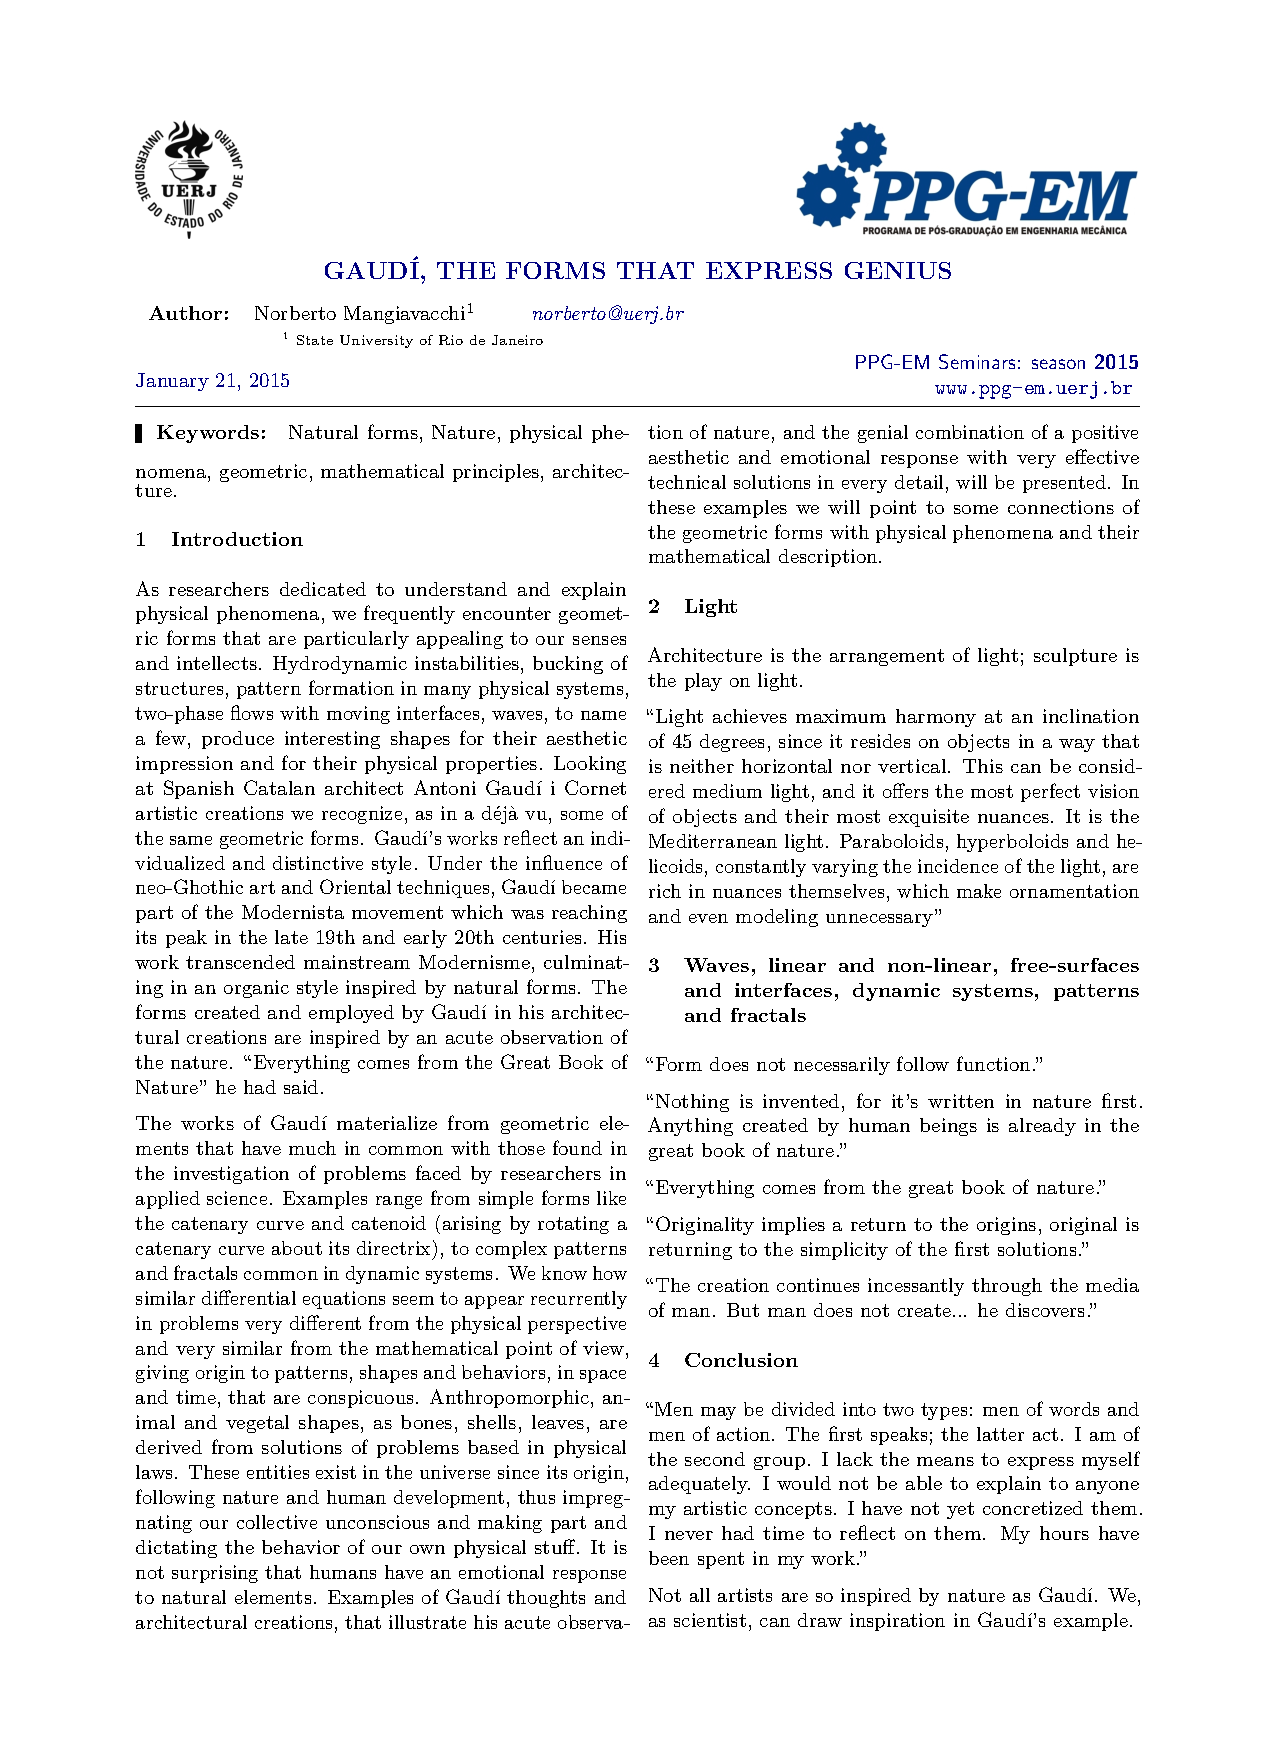
\includepdf[pages={1-2}]{../papers_pdf/18-19-seminario_norberto.pdf}
%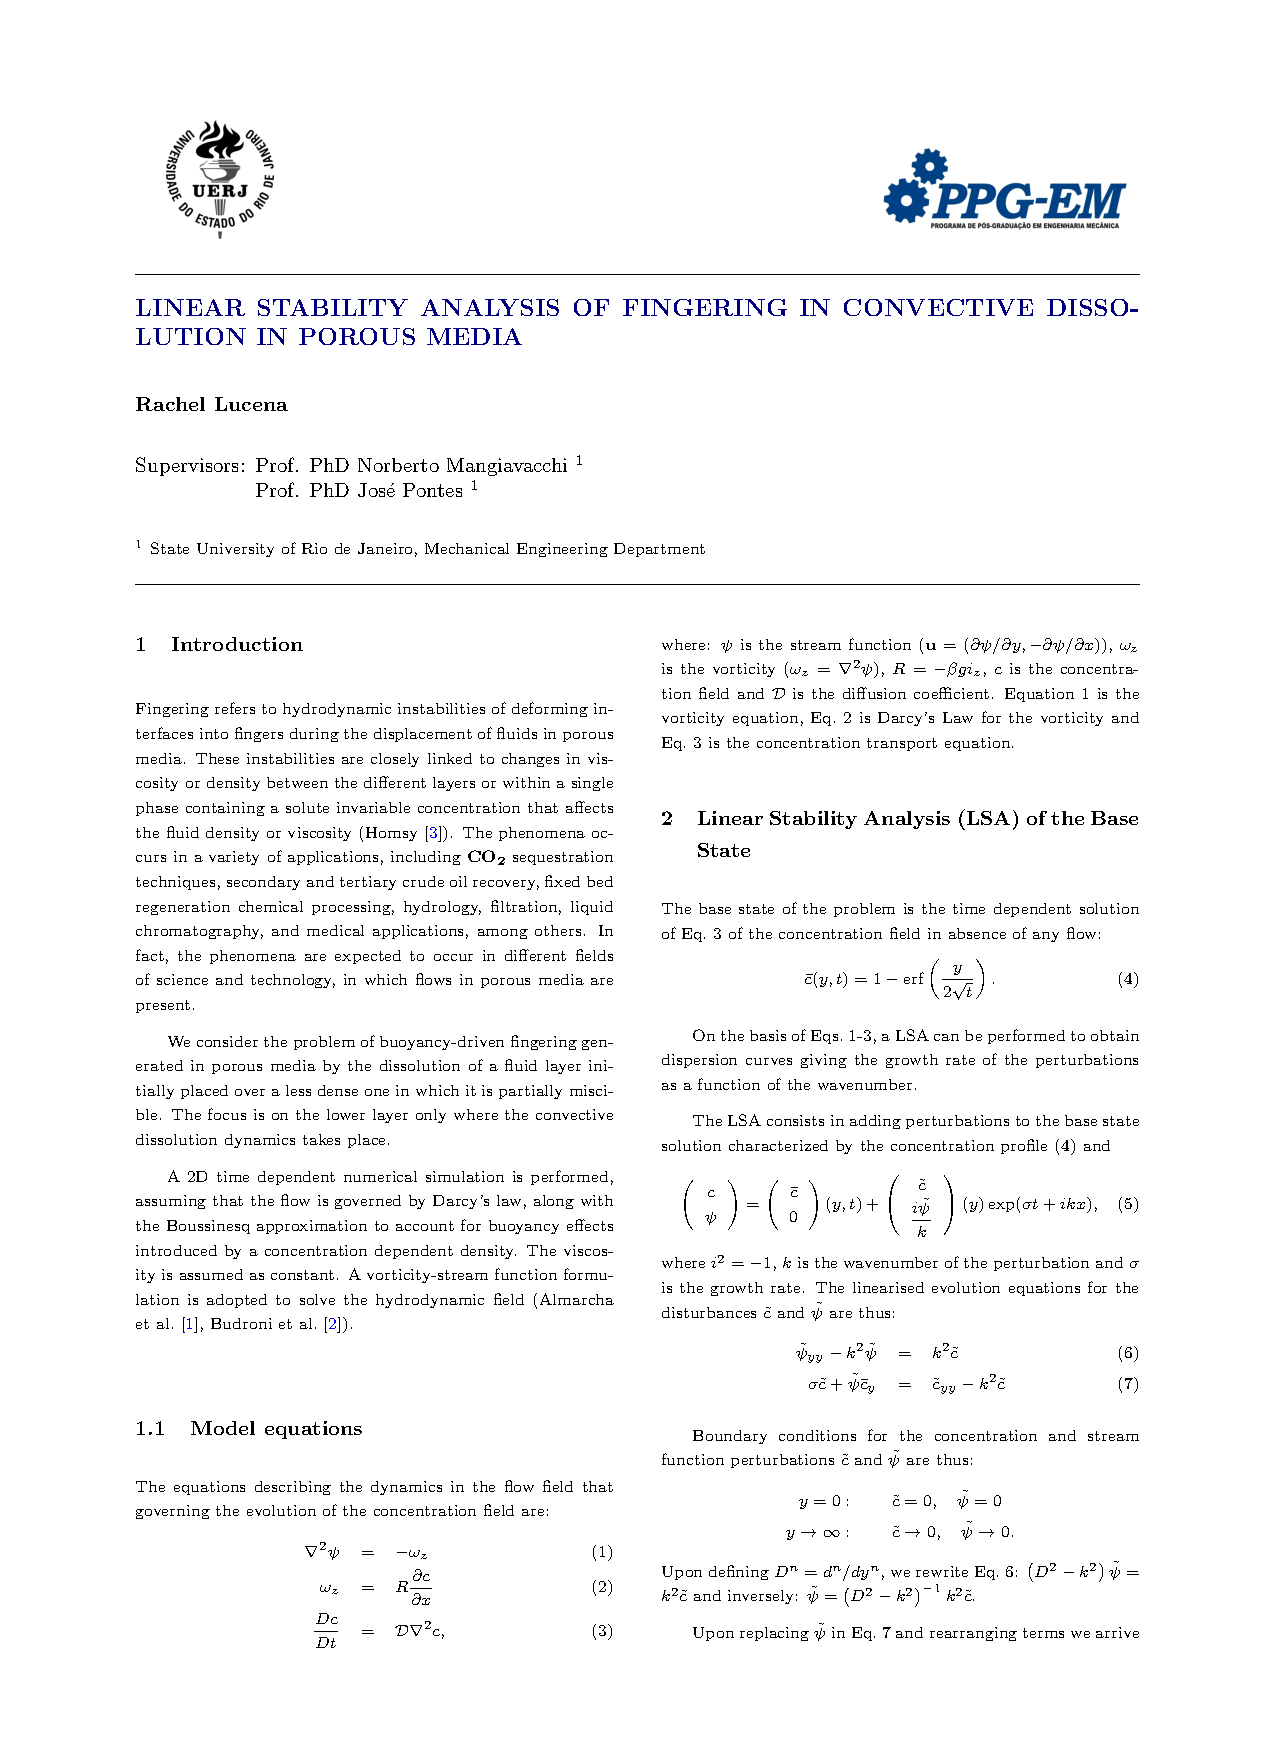
\includepdf[pages={1-2}]{../papers_pdf/20-21-seminario_rachel.pdf}
%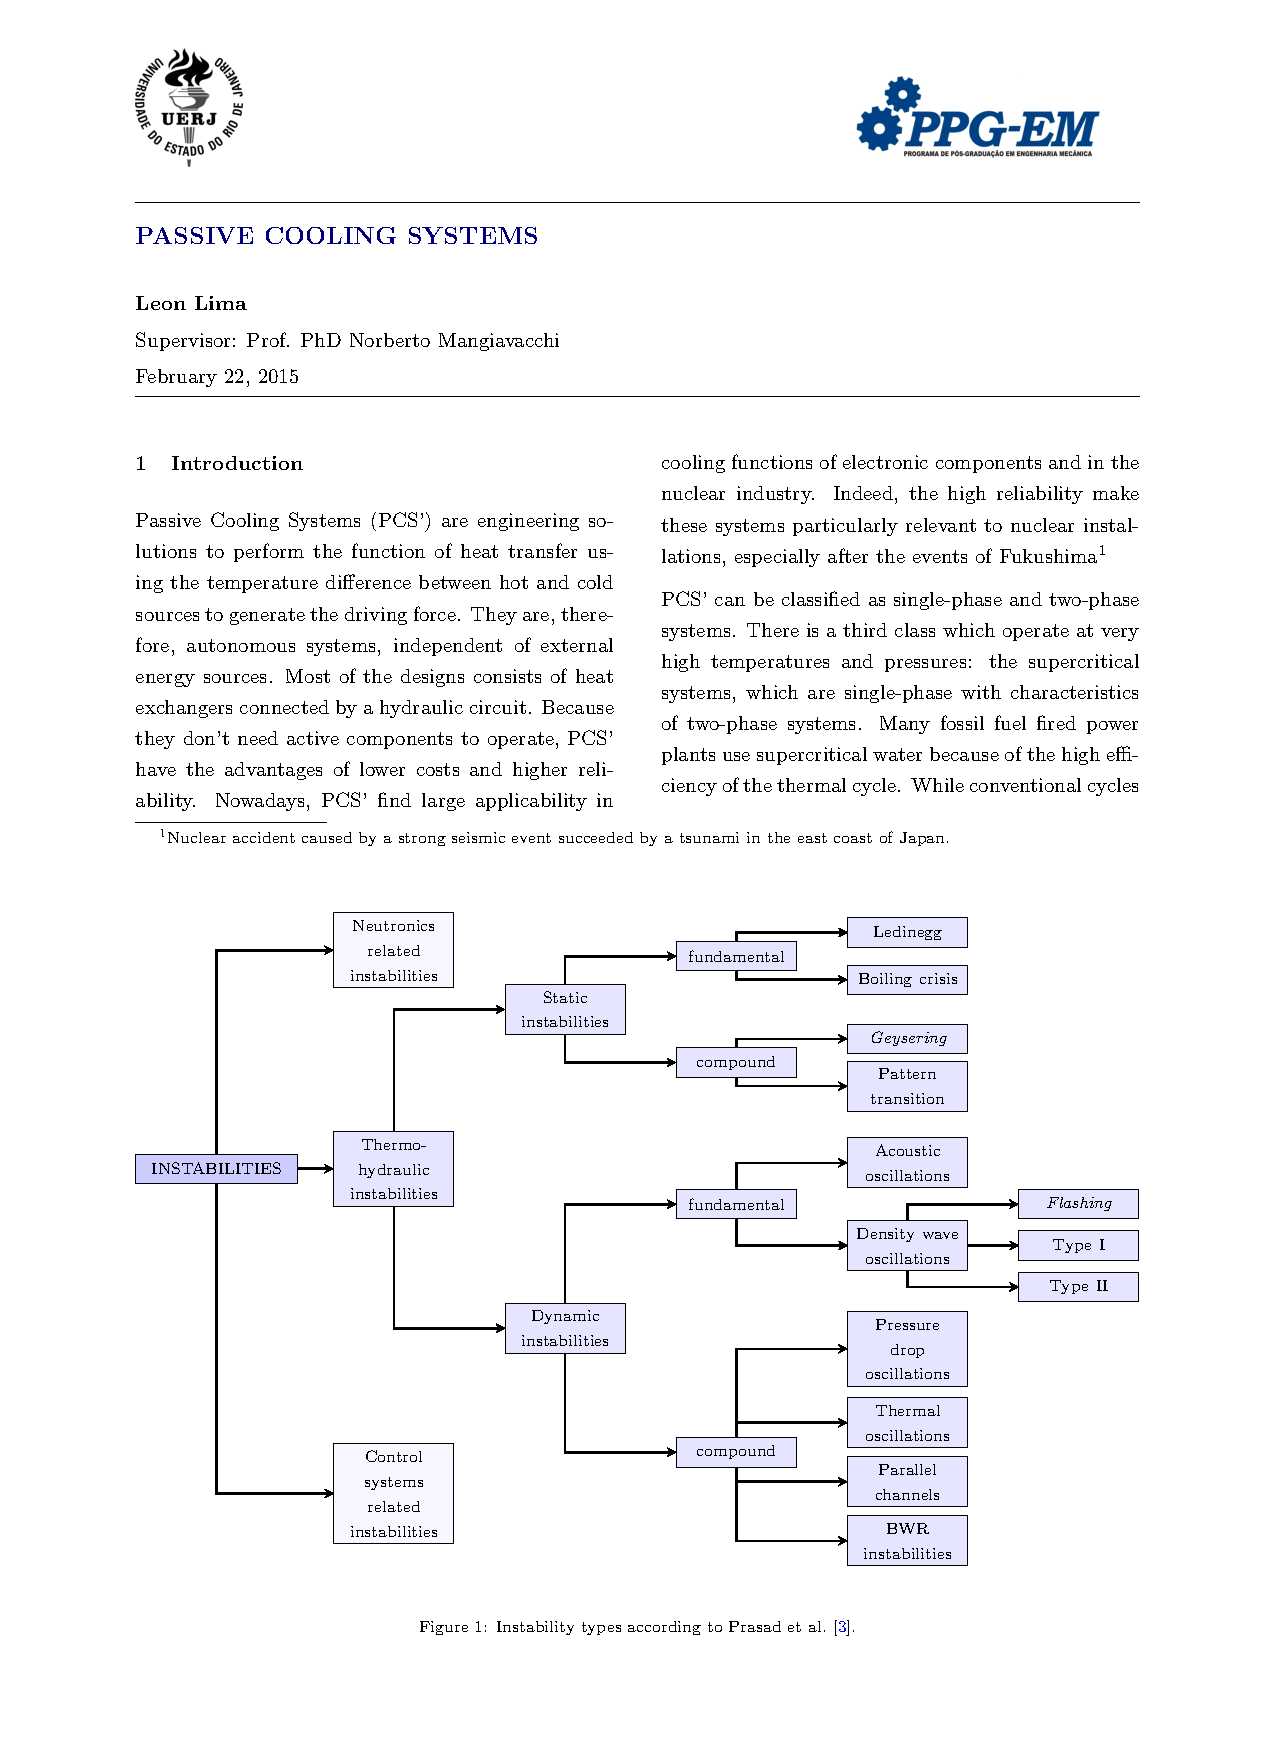
\includepdf[pages={1-2}]{../papers_pdf/22-23-seminario_leon.pdf}
%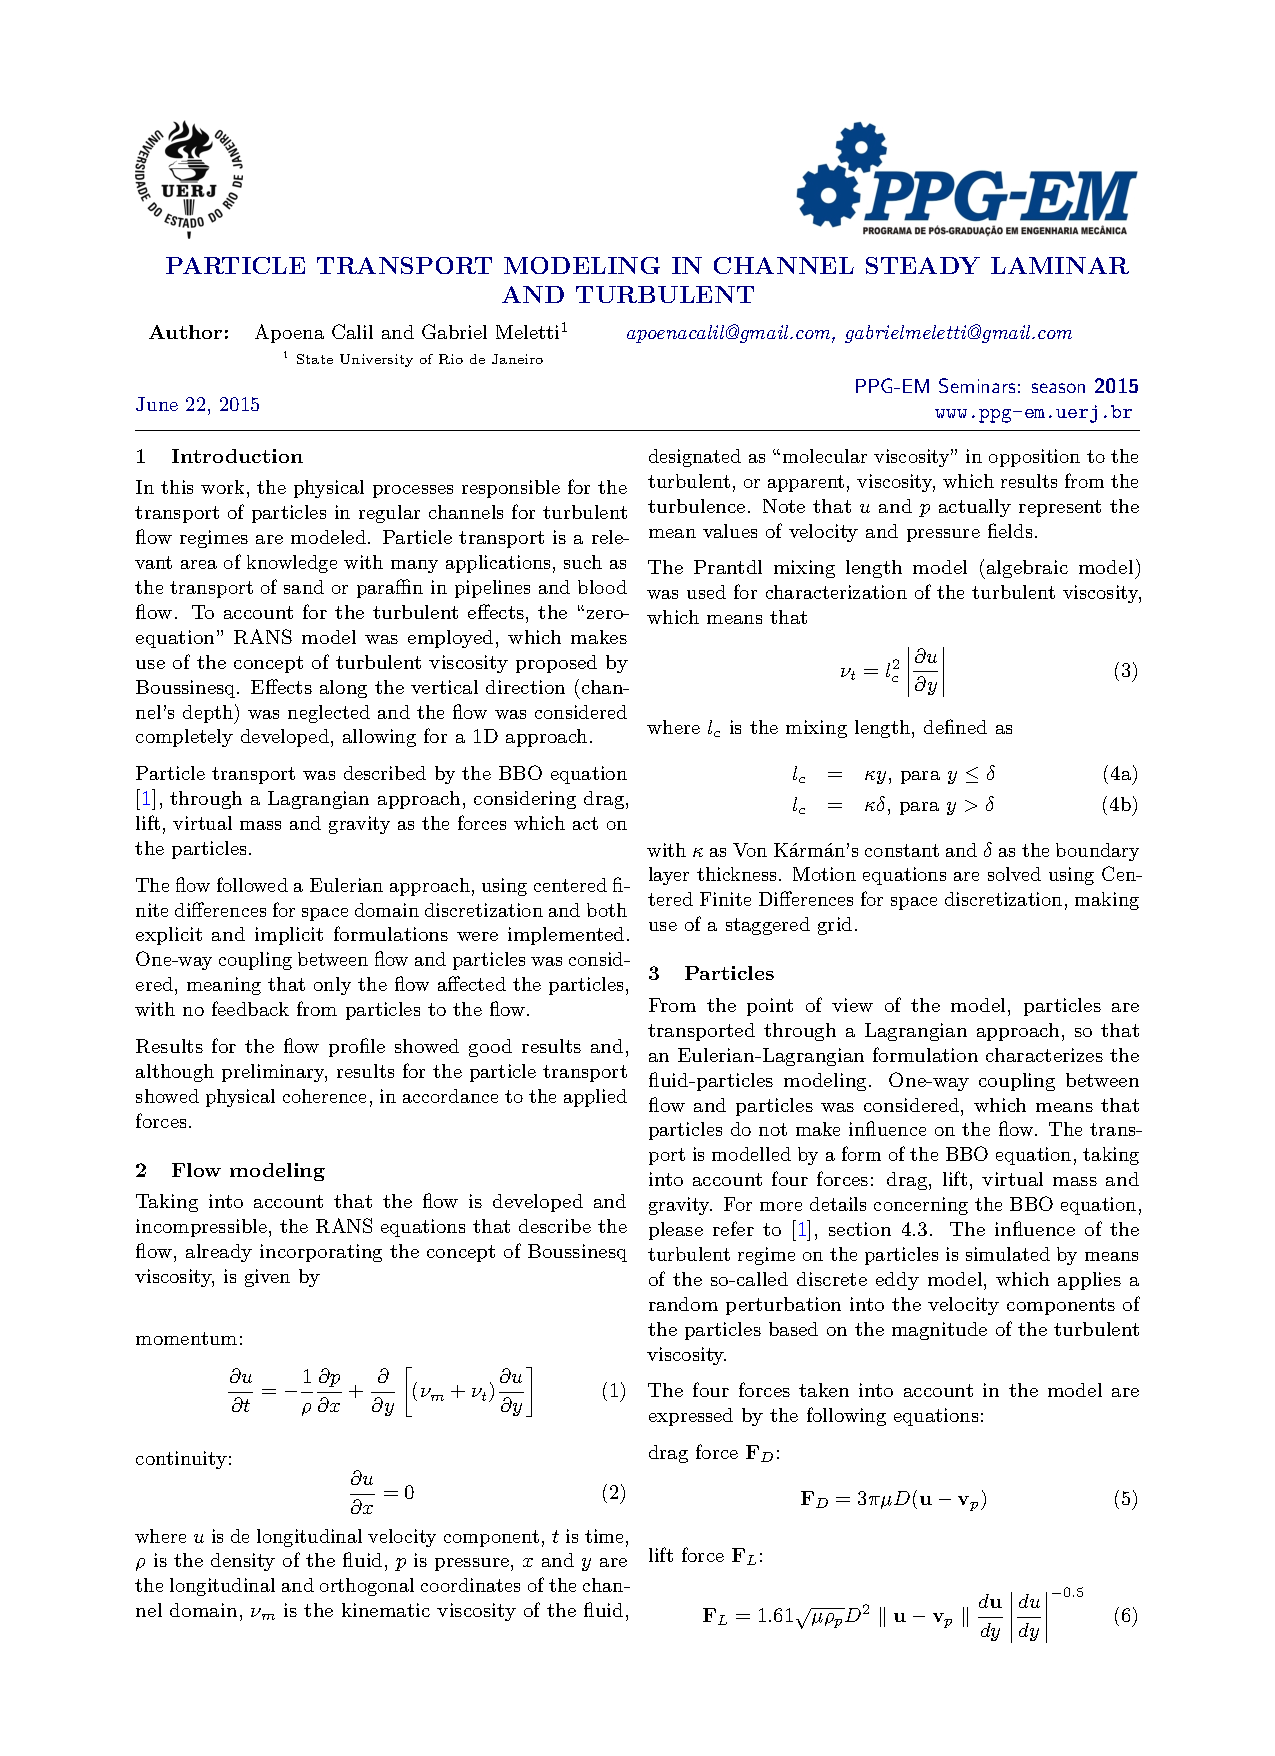
\includepdf[pages={1-2}]{../papers_pdf/24-25-seminario_apoena_gabriel.pdf}
%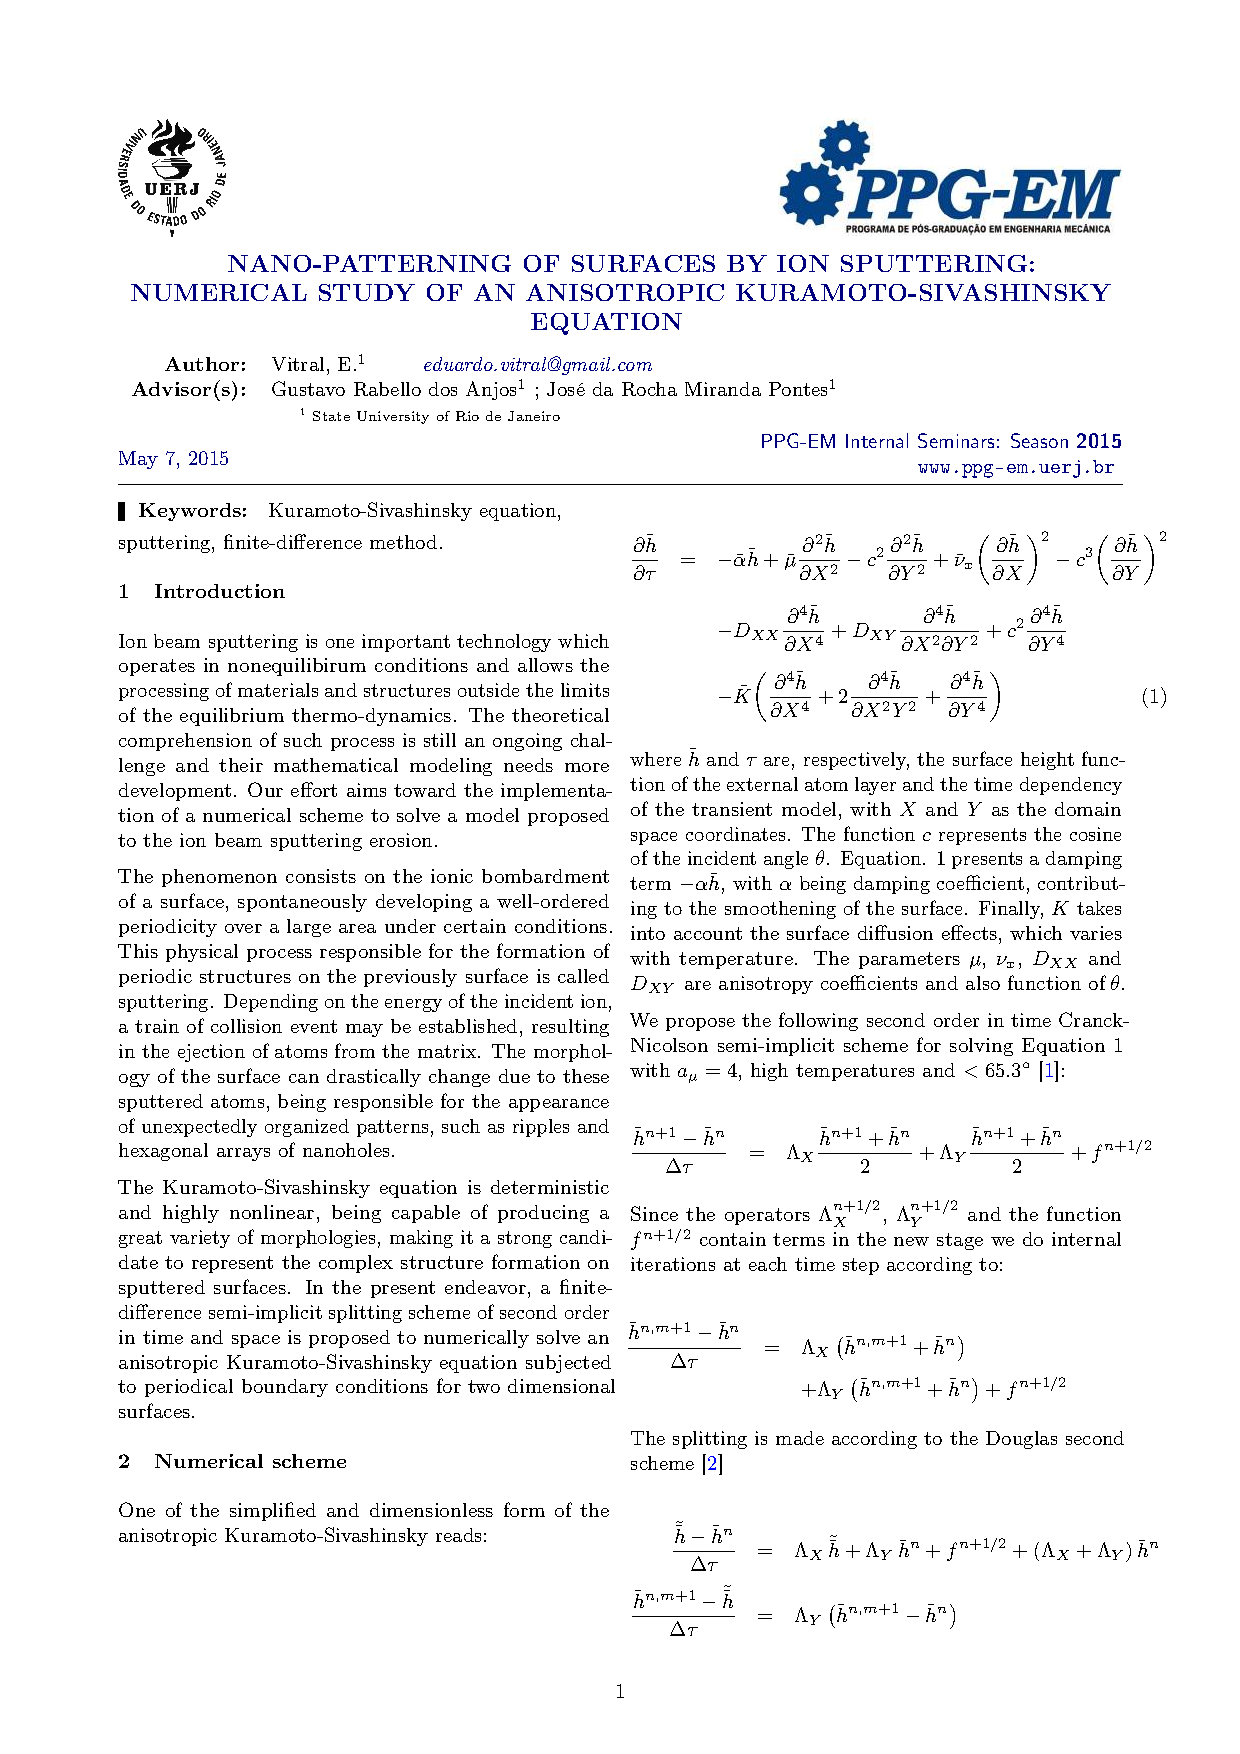
\includepdf[pages={1-2}]{../papers_pdf/26-27-seminario_eduardo.pdf}
%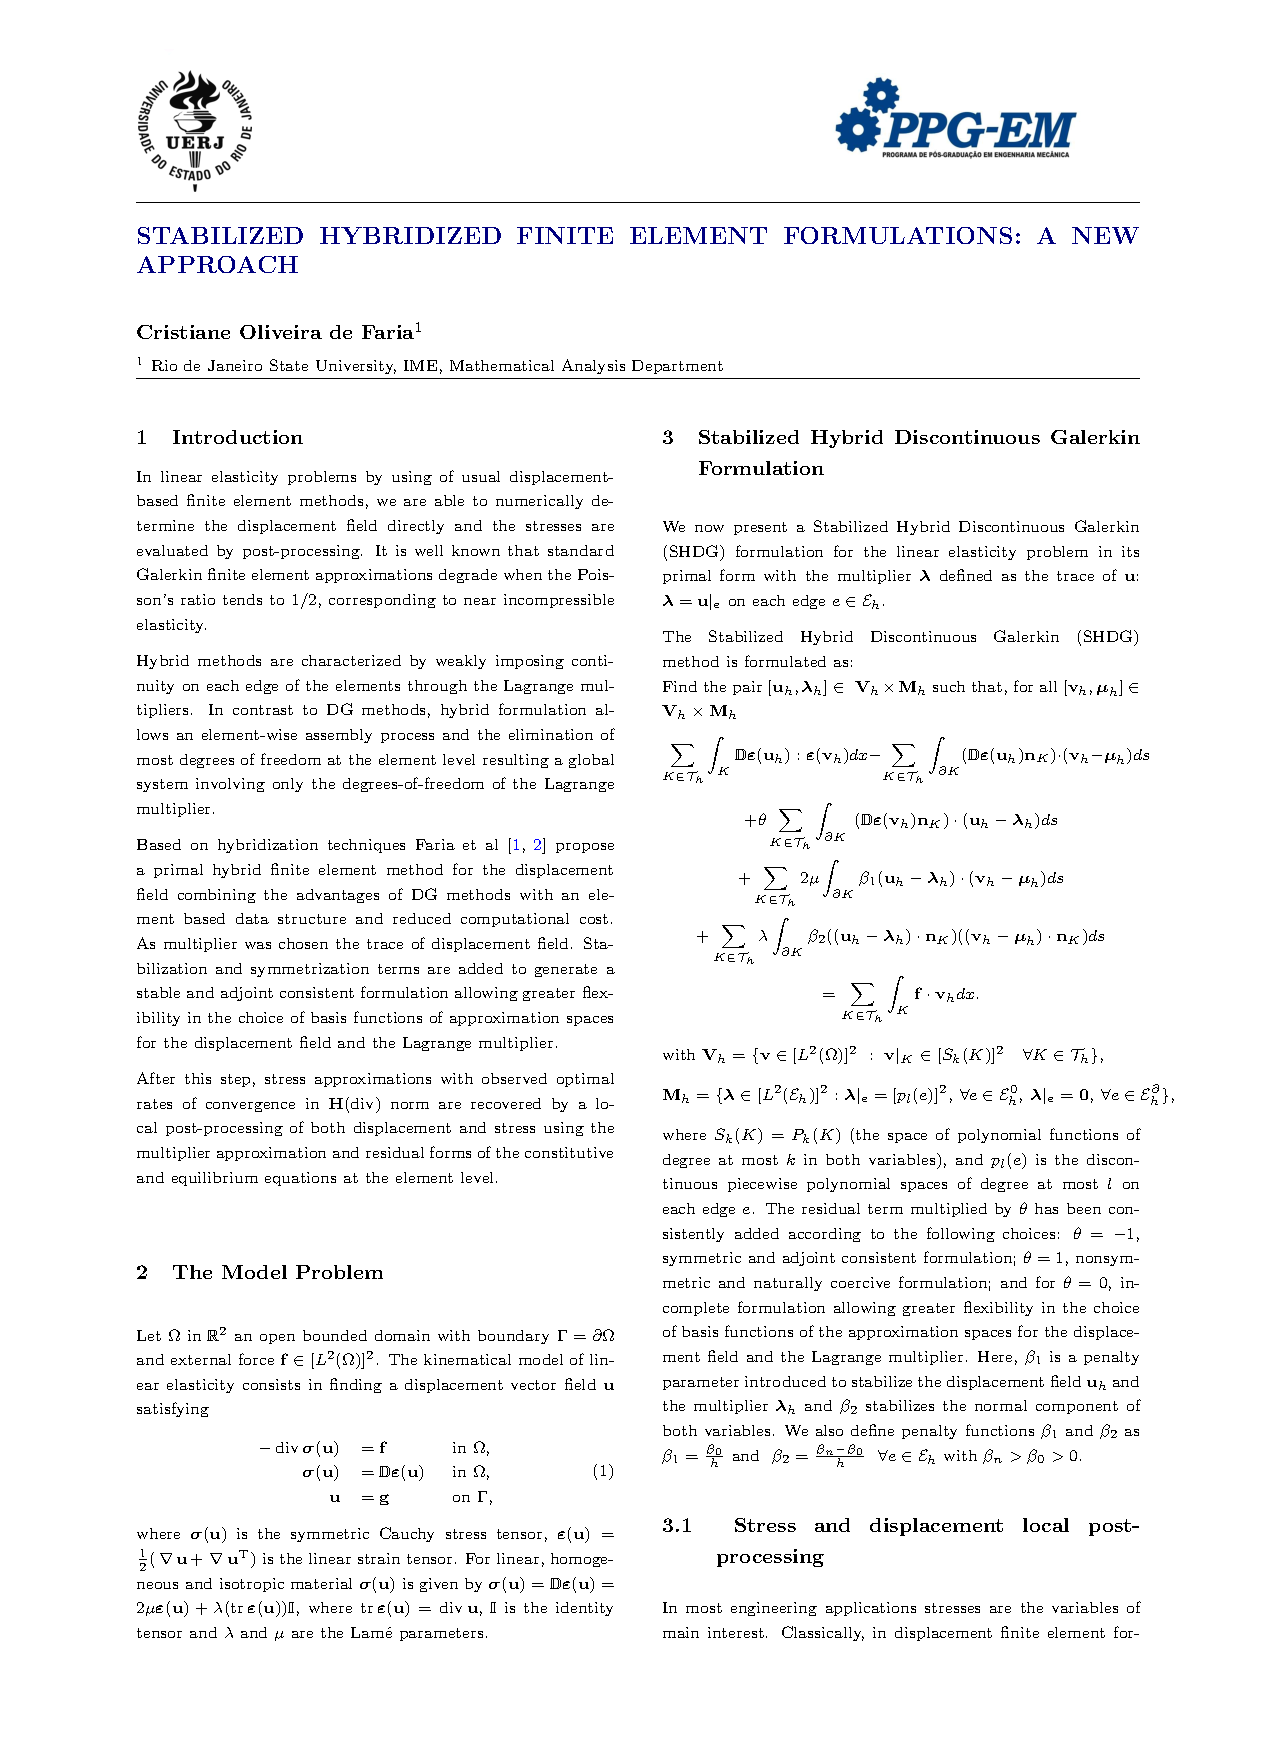
\includepdf[pages={1-2}]{../papers_pdf/28-29-seminario_cristiane.pdf}
%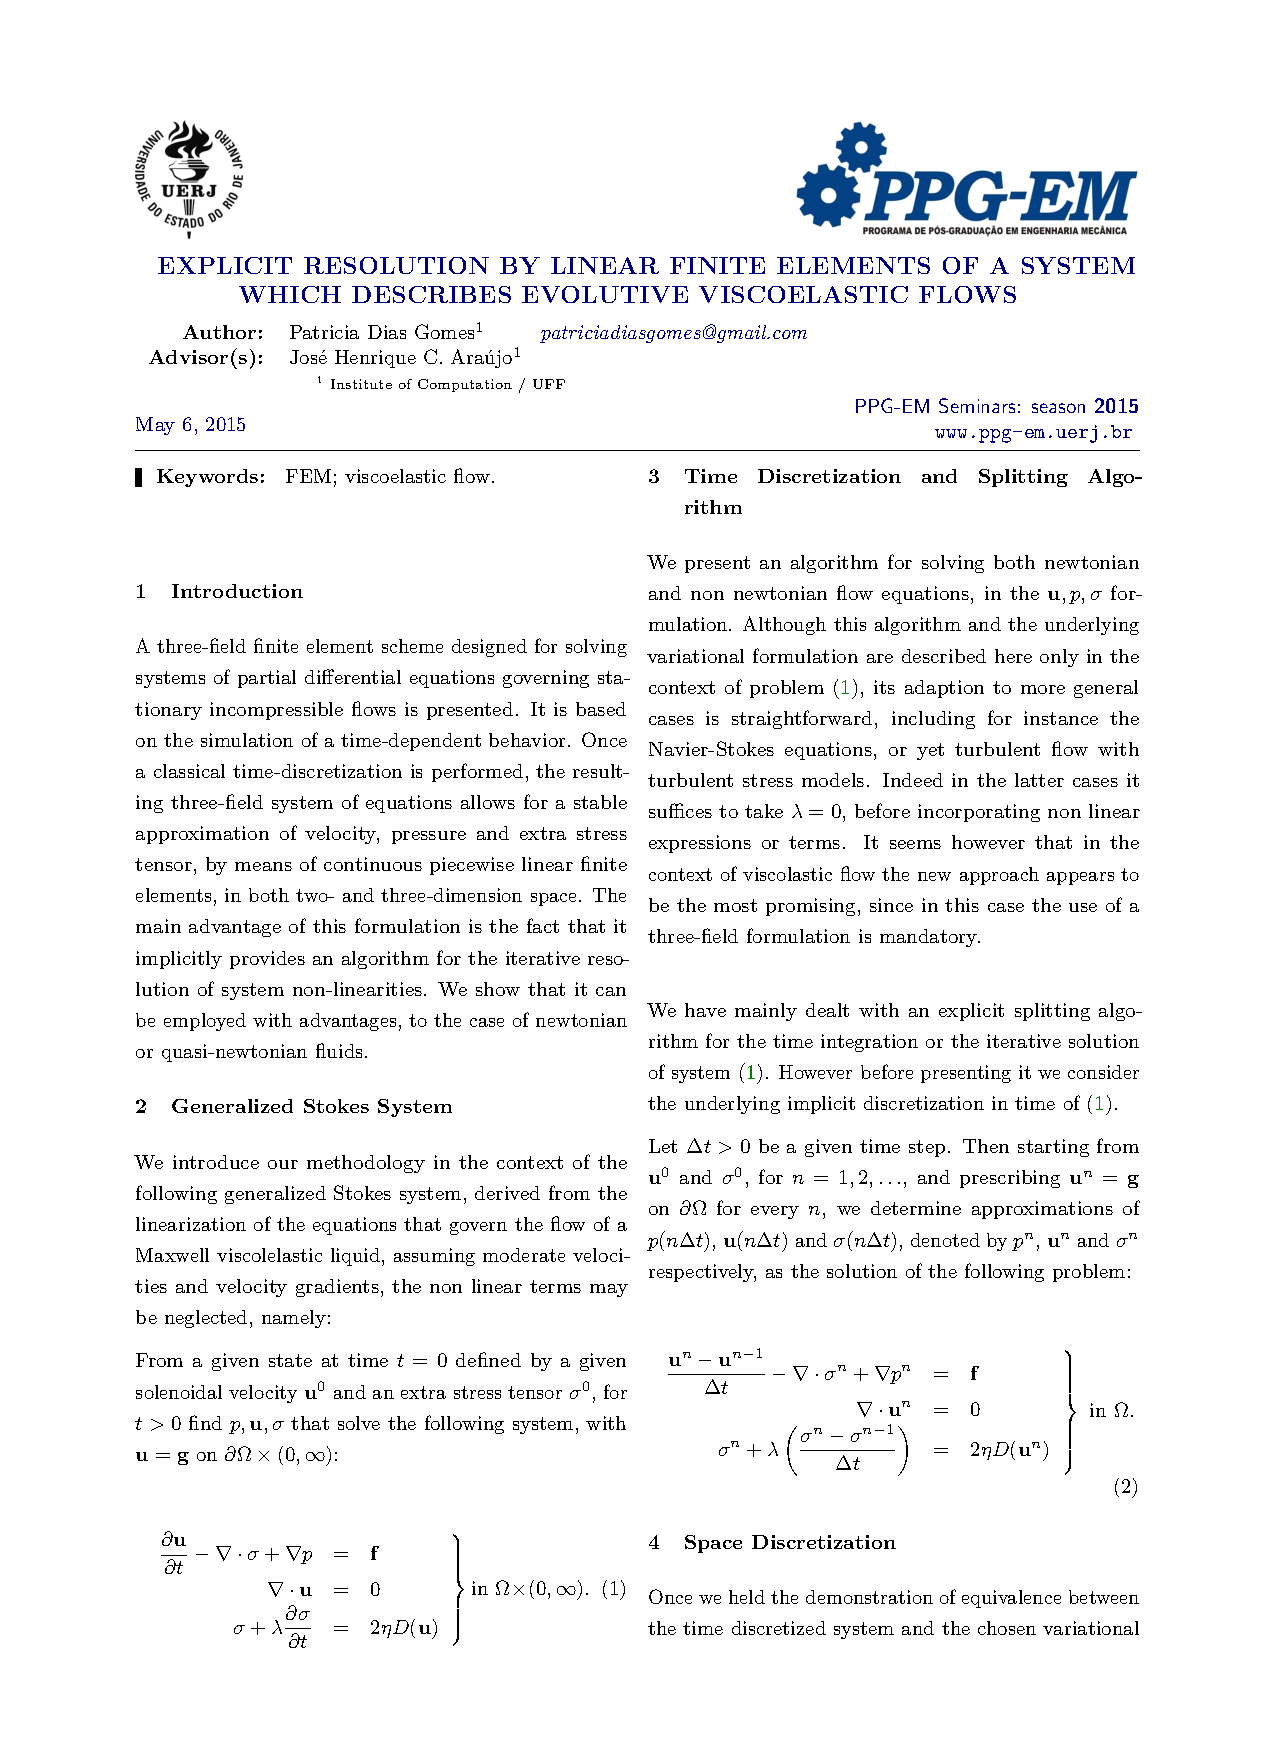
\includepdf[pages={1-2}]{../papers_pdf/30-31-seminario_patricia.pdf}
%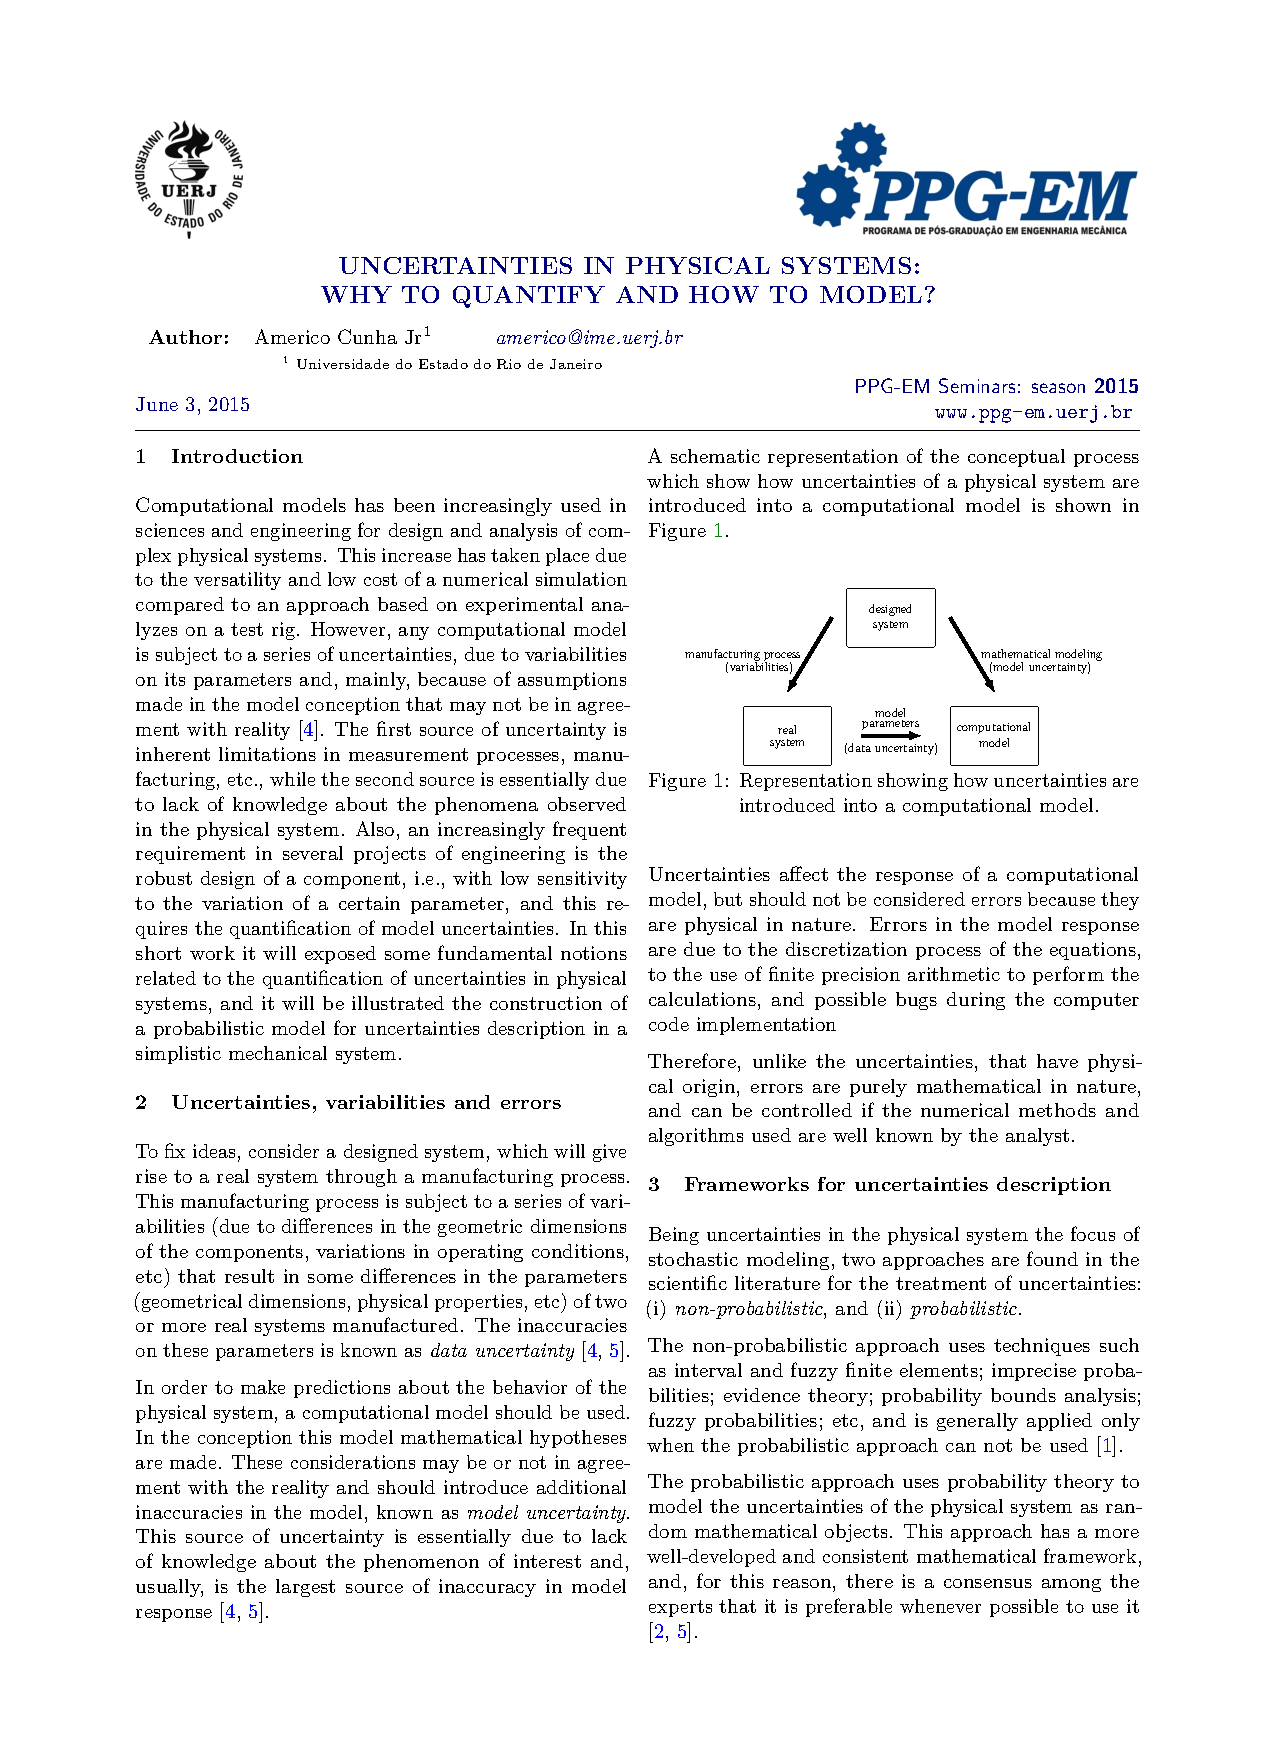
\includepdf[pages={1-2}]{../papers_pdf/32-33-seminario_americo.pdf}
%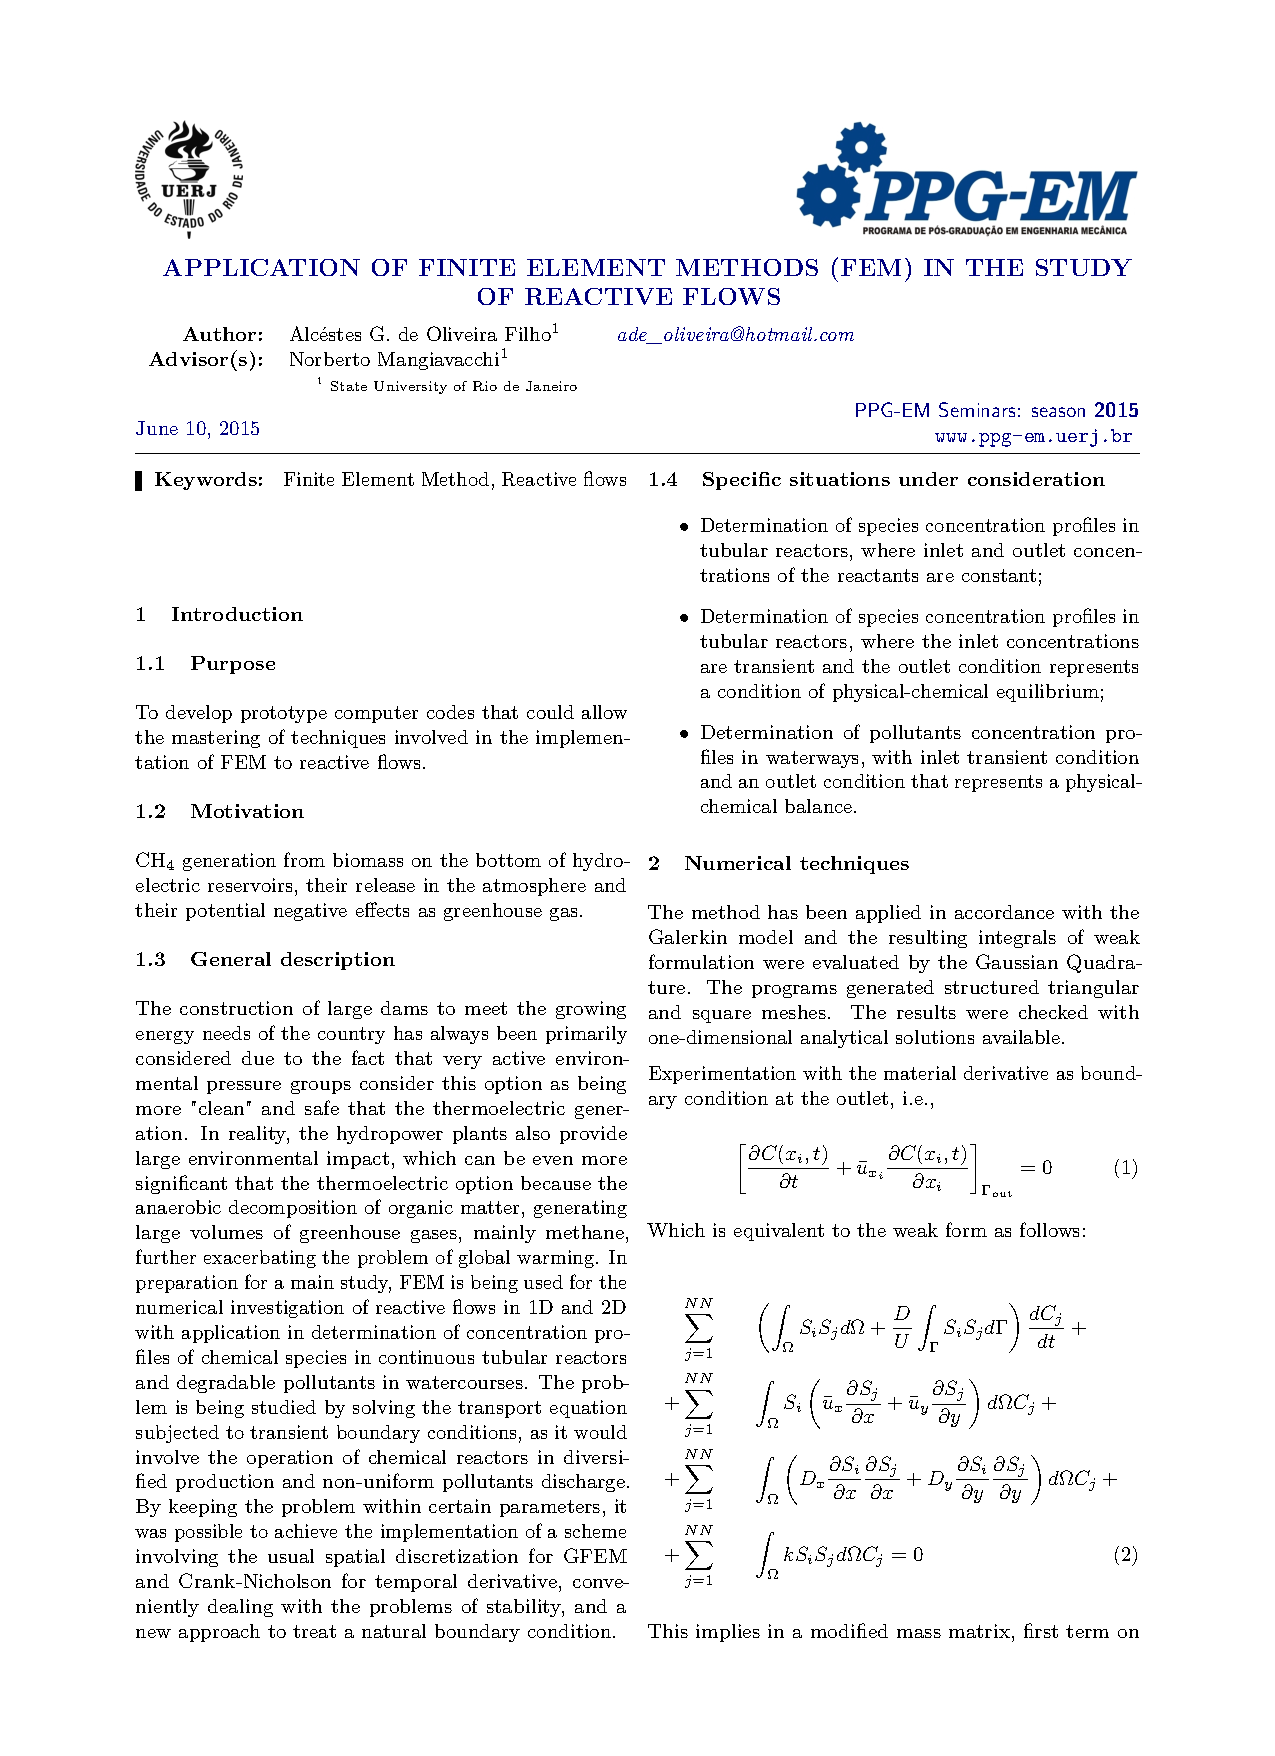
\includepdf[pages={1-2}]{../papers_pdf/34-35-seminario_alcestes.pdf}
%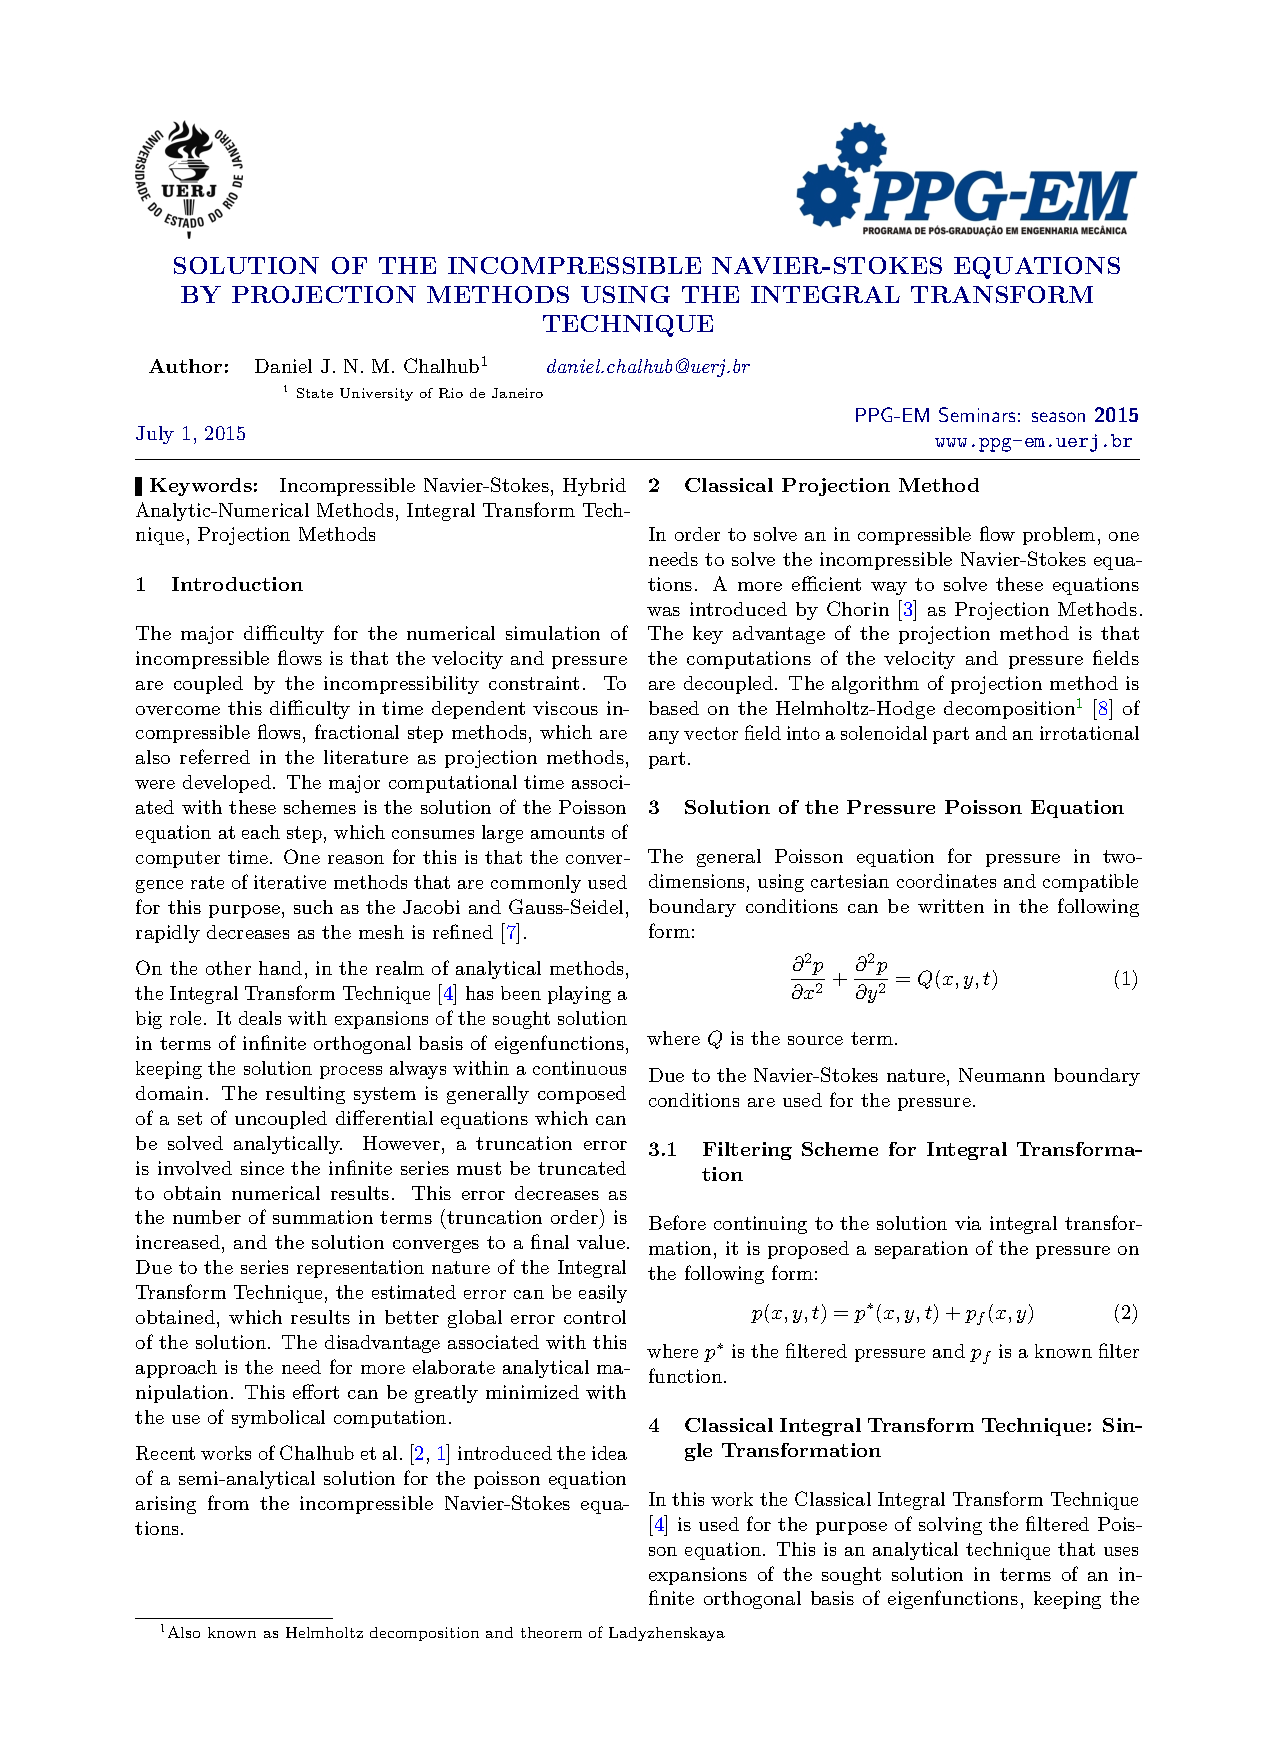
\includepdf[pages={1-2}]{../papers_pdf/36-37-seminario_daniel.pdf}
%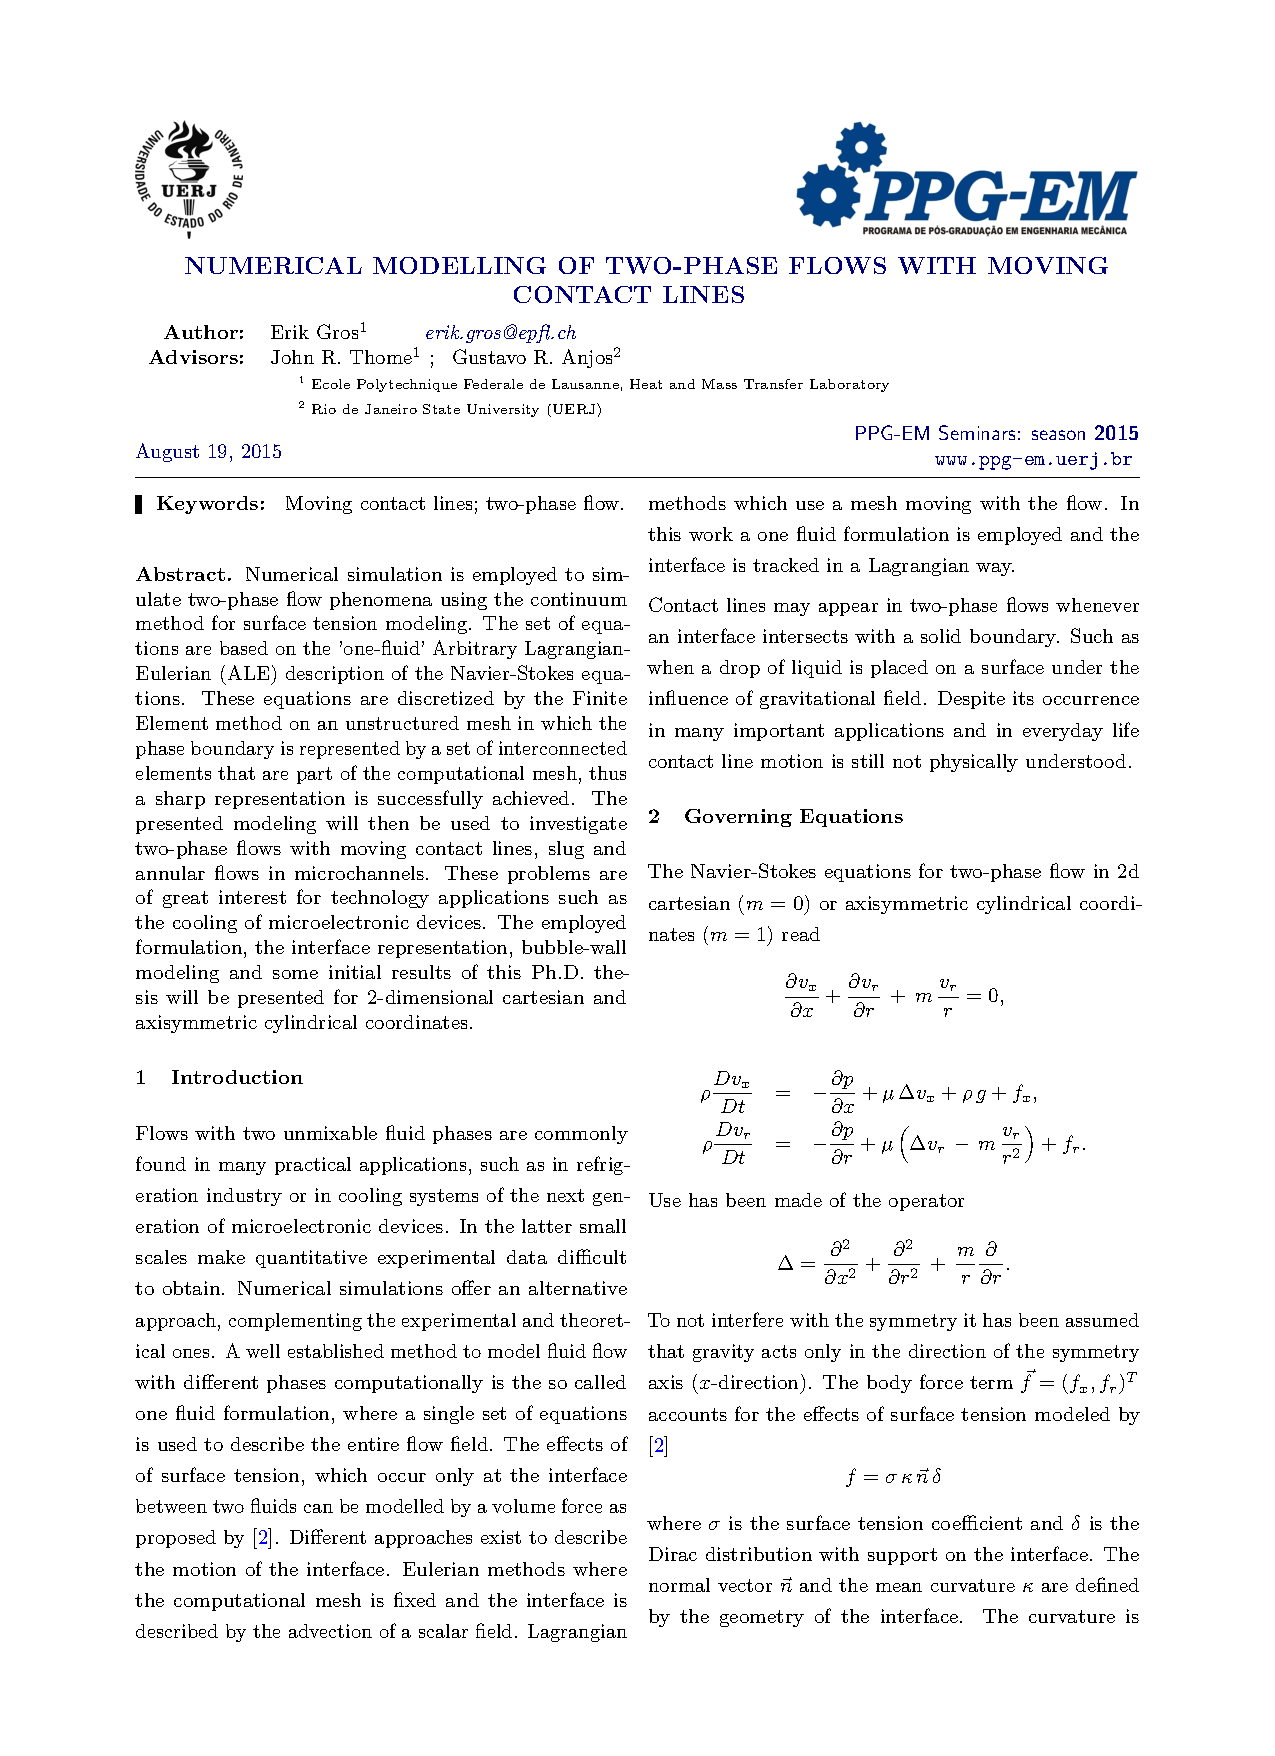
\includepdf[pages={1-2}]{../papers_pdf/38-39-seminario_erik.pdf}
%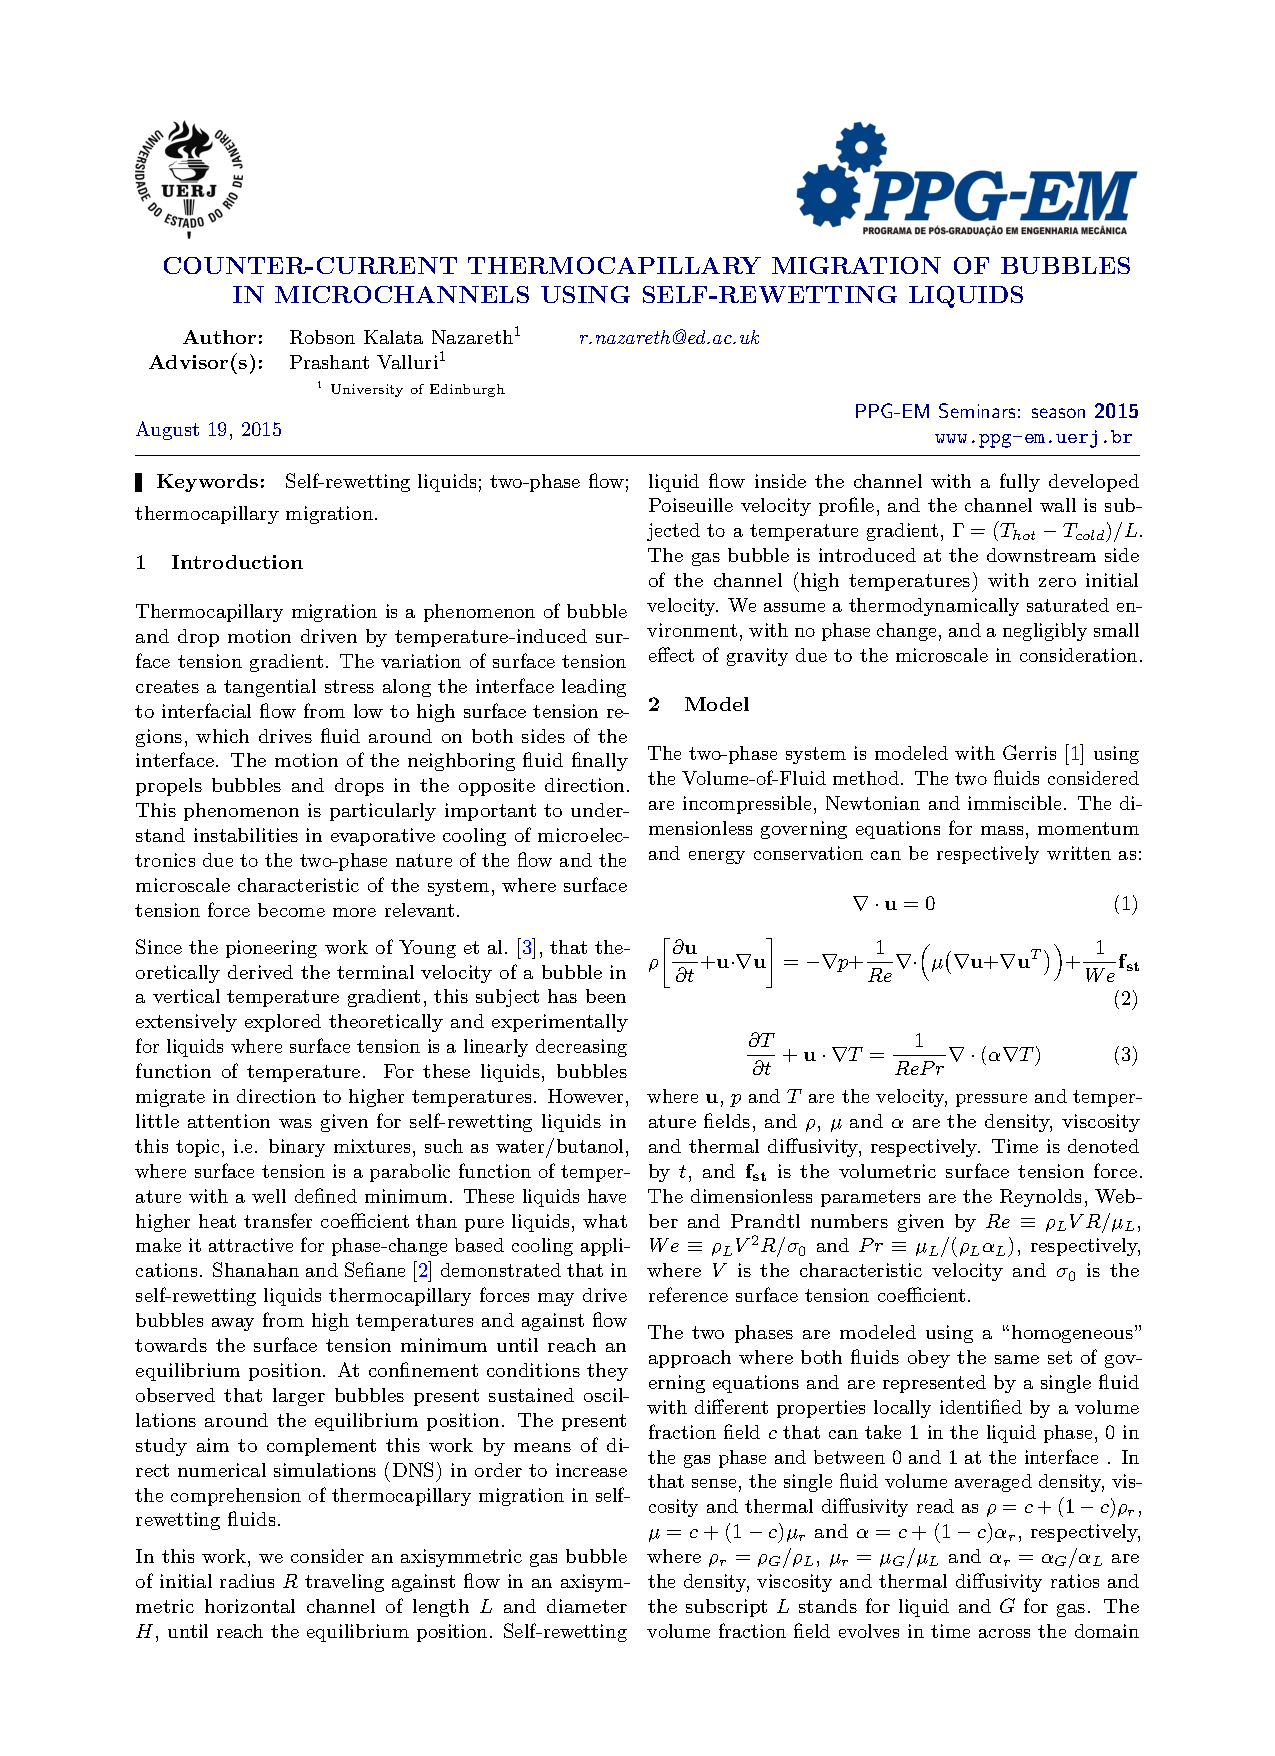
\includepdf[pages={1-2}]{../papers_pdf/40-41-seminario_robson.pdf}
%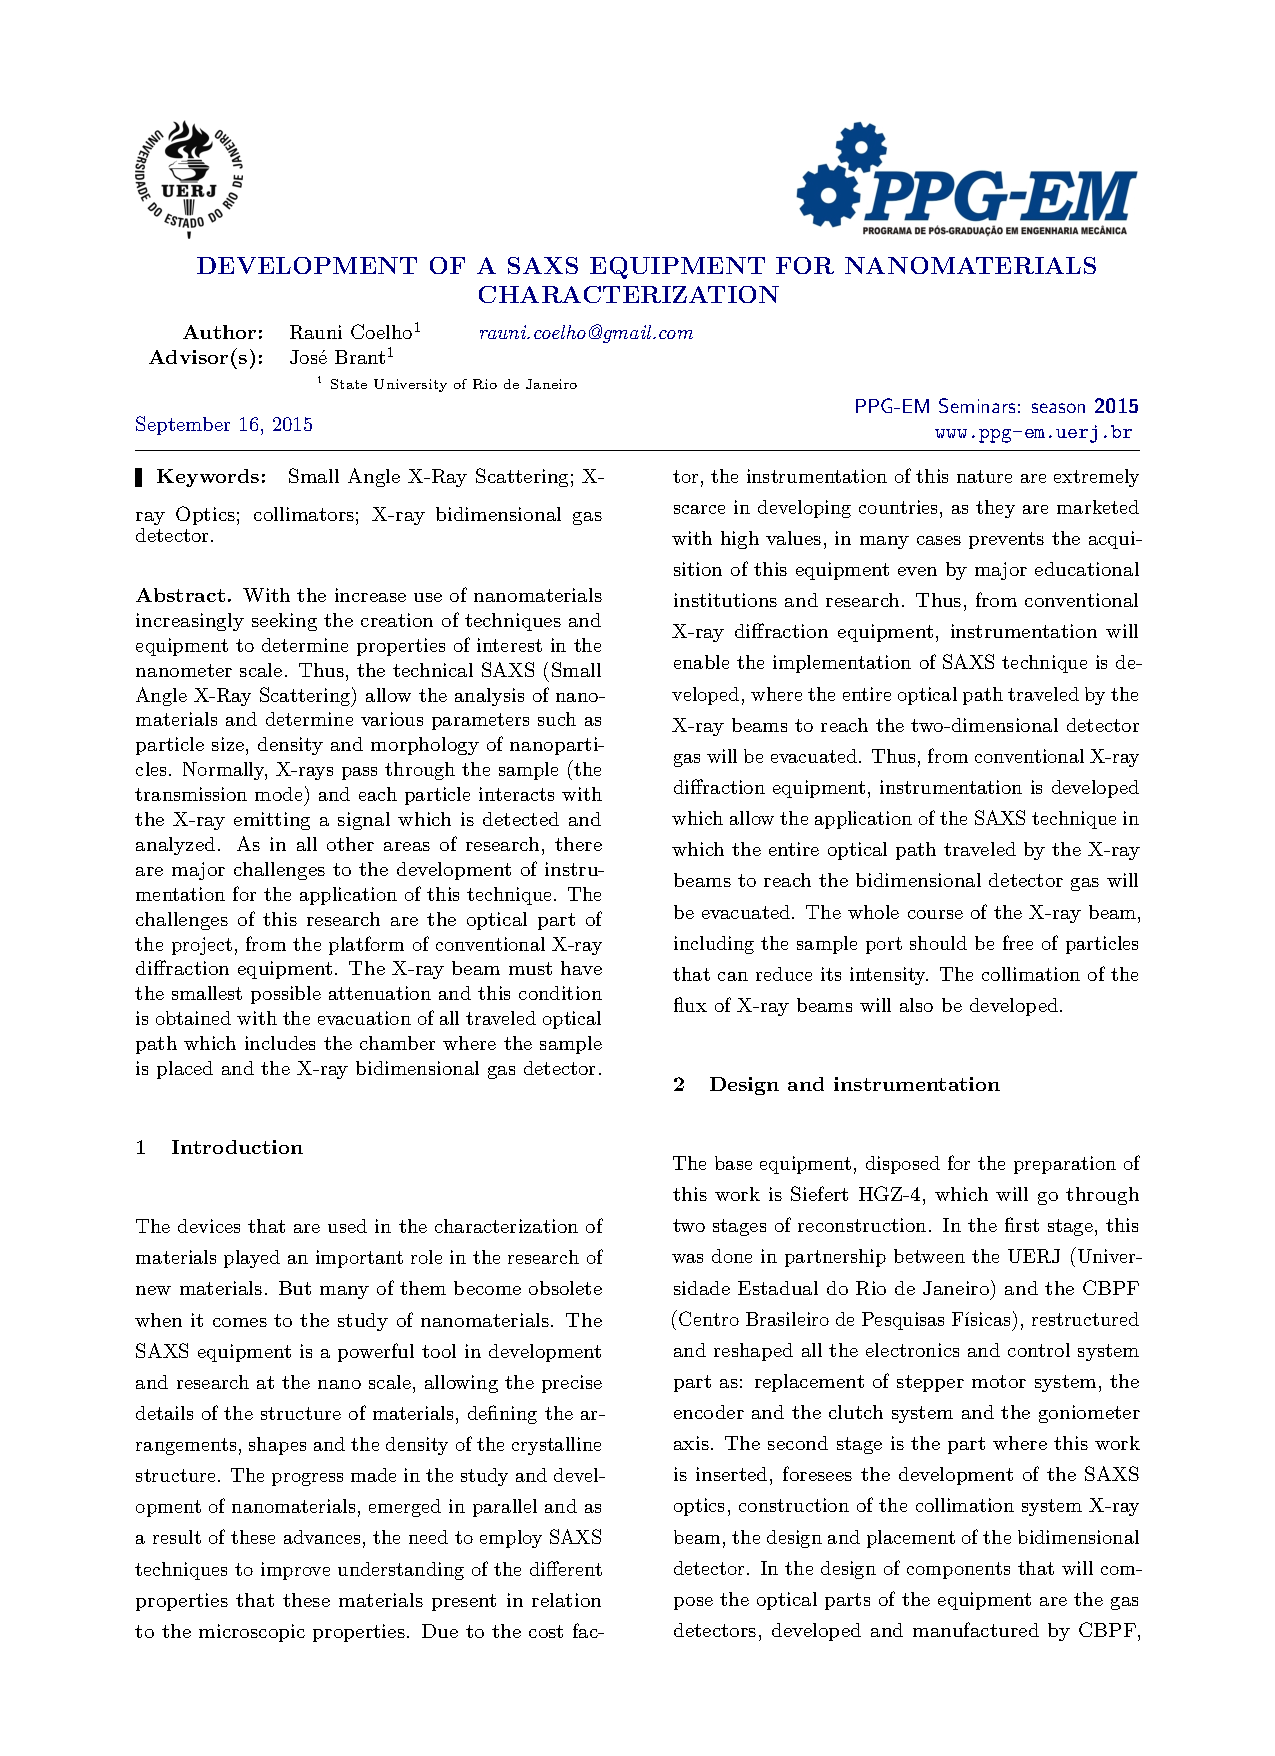
\includepdf[pages={1-2}]{../papers_pdf/42-43-seminario_rauni.pdf}
%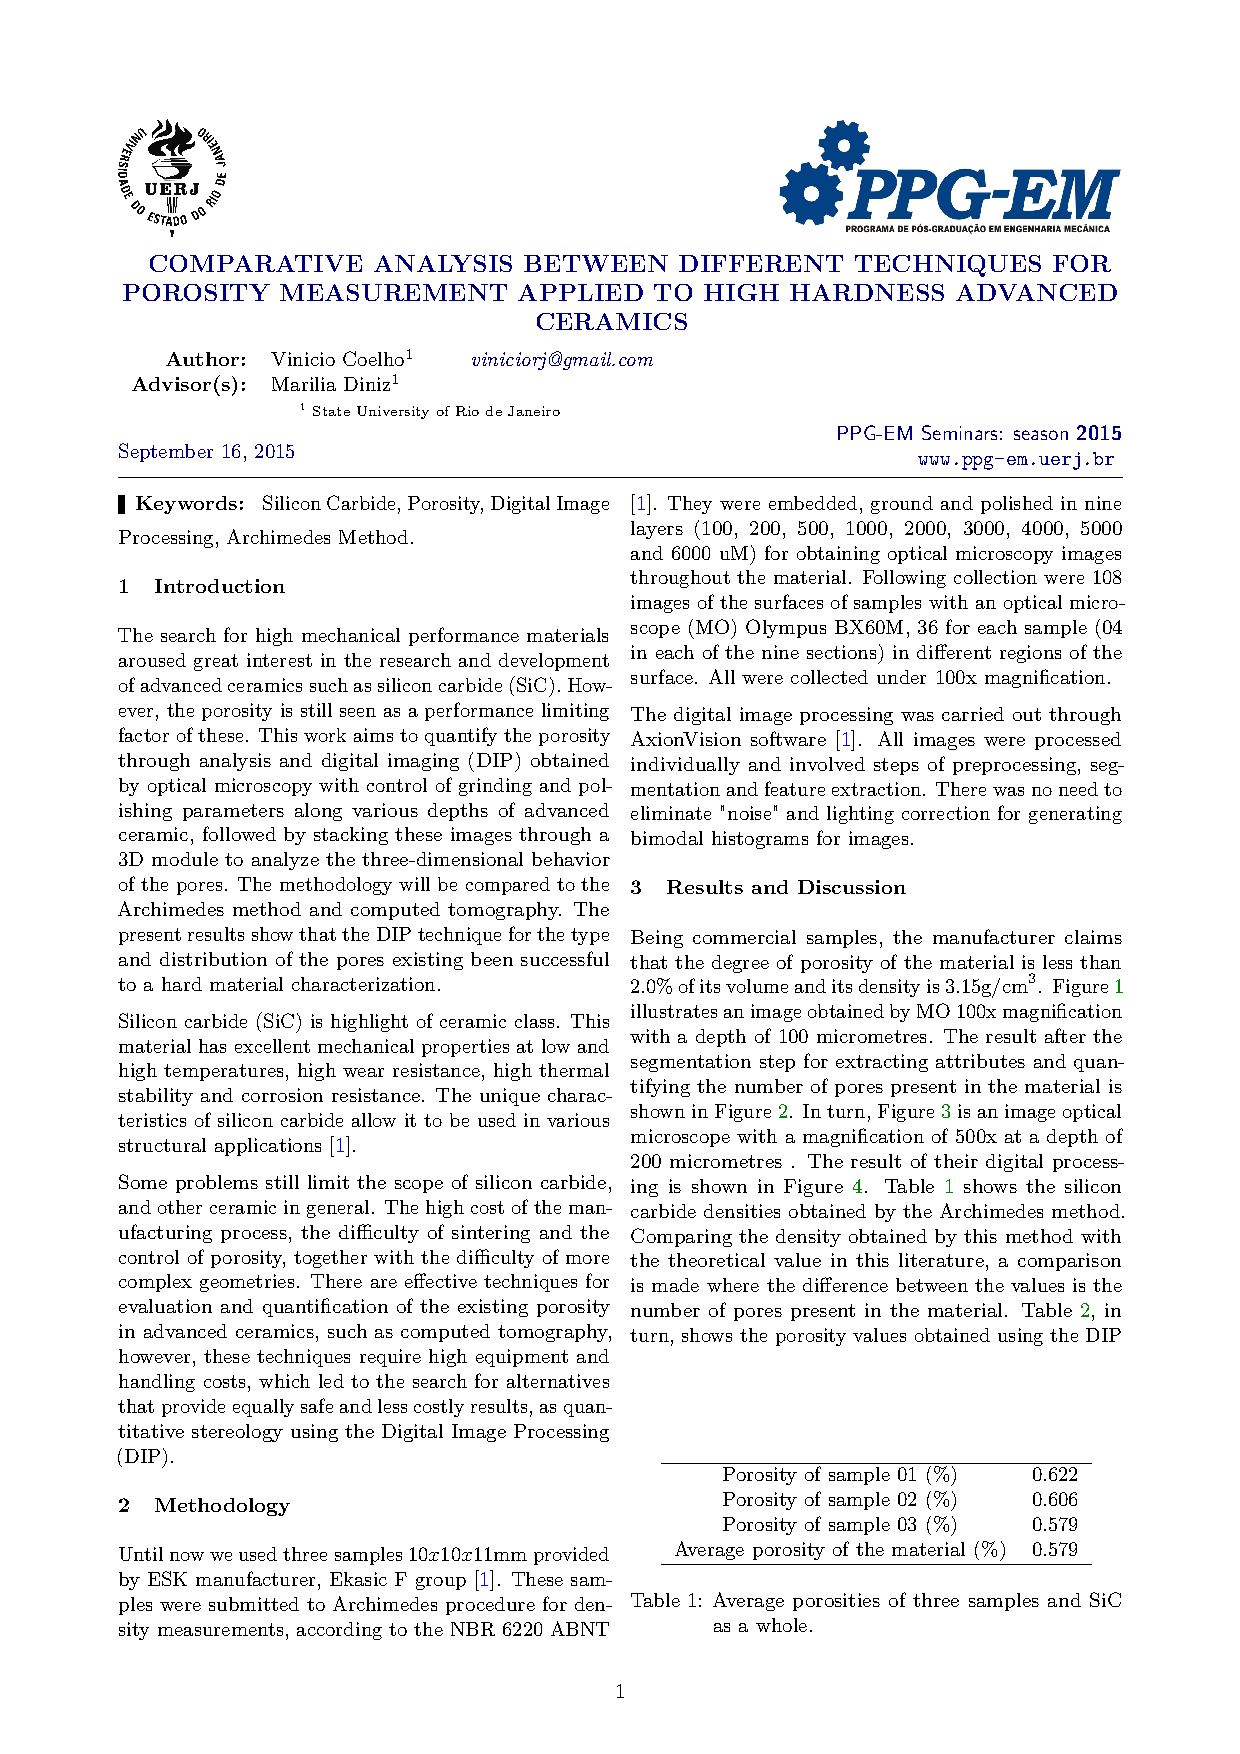
\includepdf[pages={1-2}]{../papers_pdf/44-45-seminario_vinicio.pdf}
%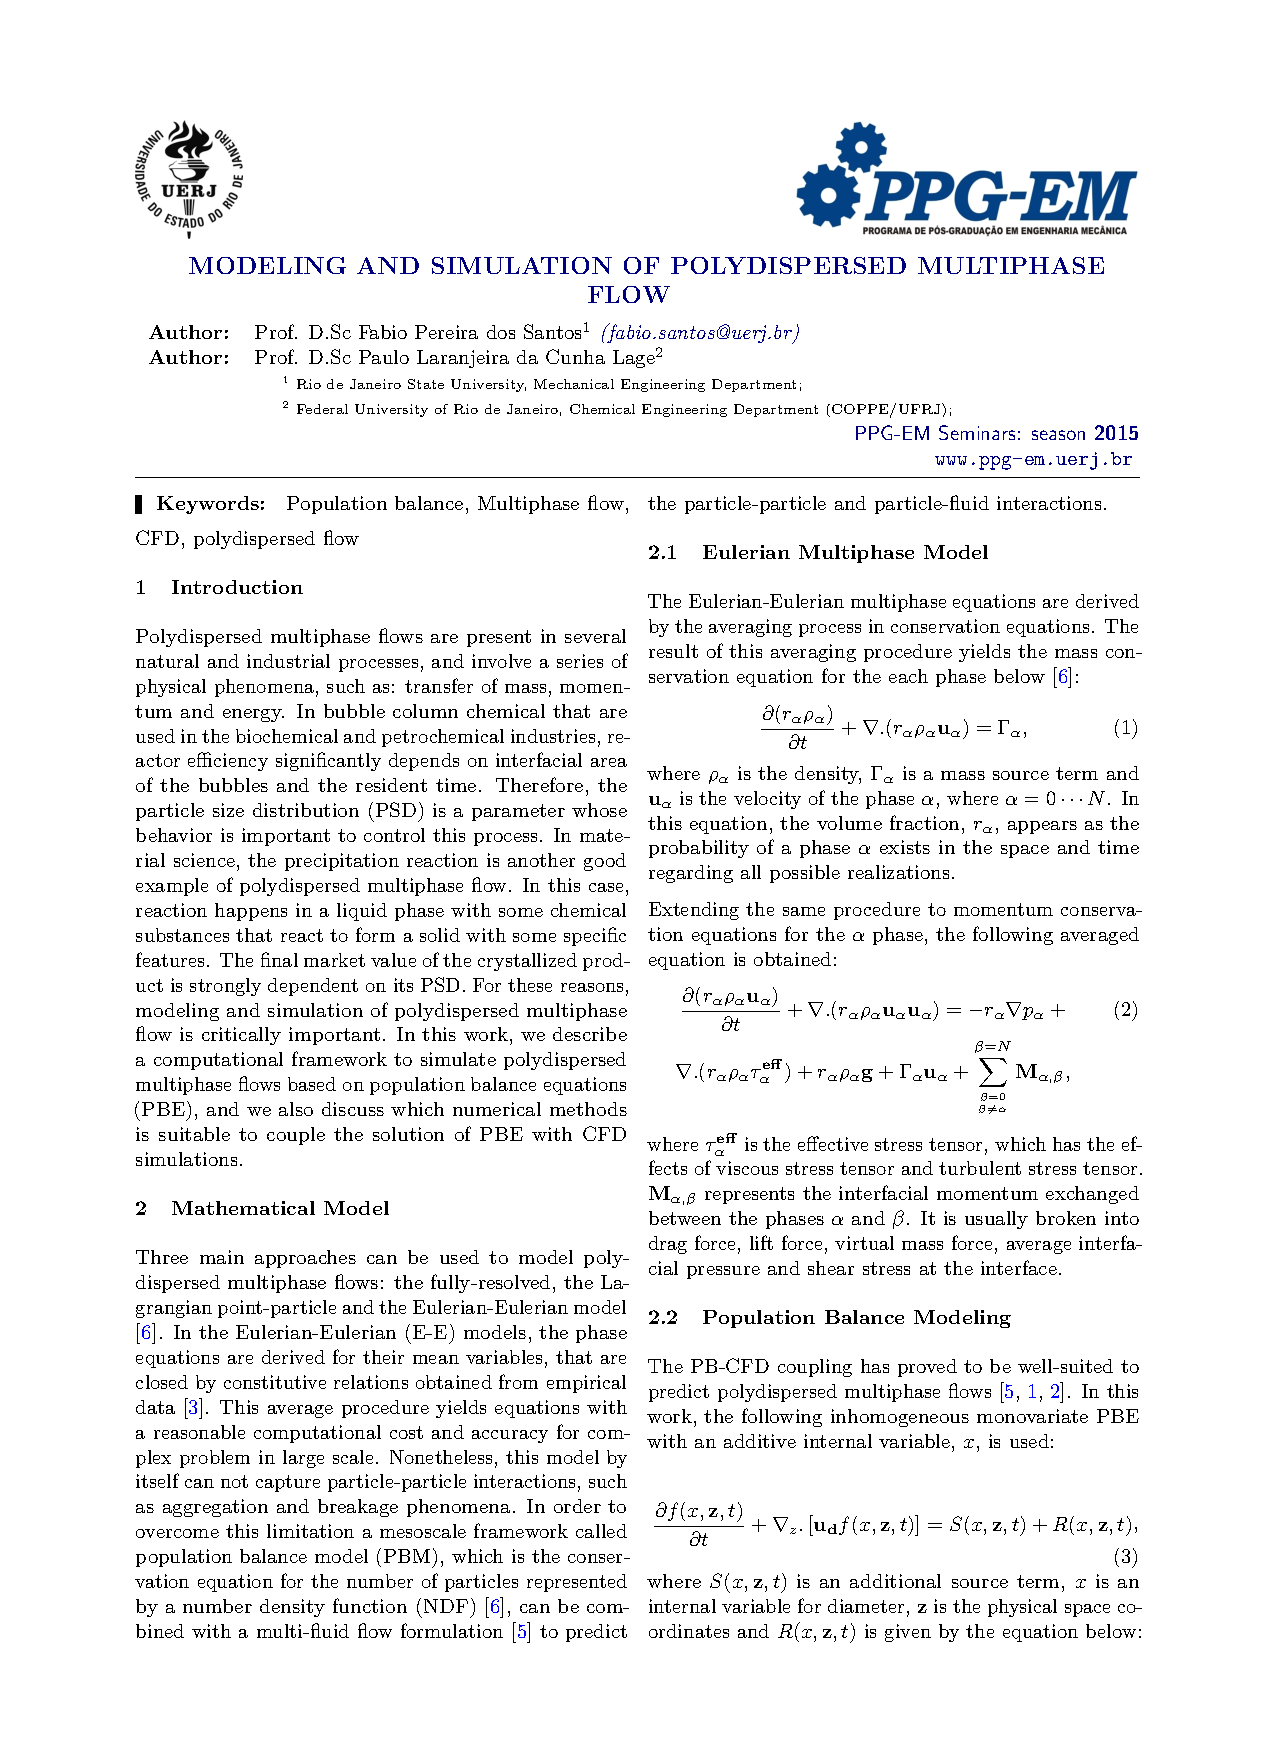
\includepdf[pages={1-2}]{../papers_pdf/46-47-seminario_fabio.pdf}


\newpage
\vspace*{\fill}
\thispagestyle{empty}

\newpage
\vspace*{\fill}
\thispagestyle{empty}

\newpage
\begingroup
\thispagestyle{empty}
\begin{tikzpicture}[remember picture,overlay]
\coordinate [below=12cm] (midpoint) at (current page.north);
\node at (current page.north west)
{\begin{tikzpicture}[remember picture,overlay]
	%\node[anchor=north west,inner sep=0pt] at (0,0) {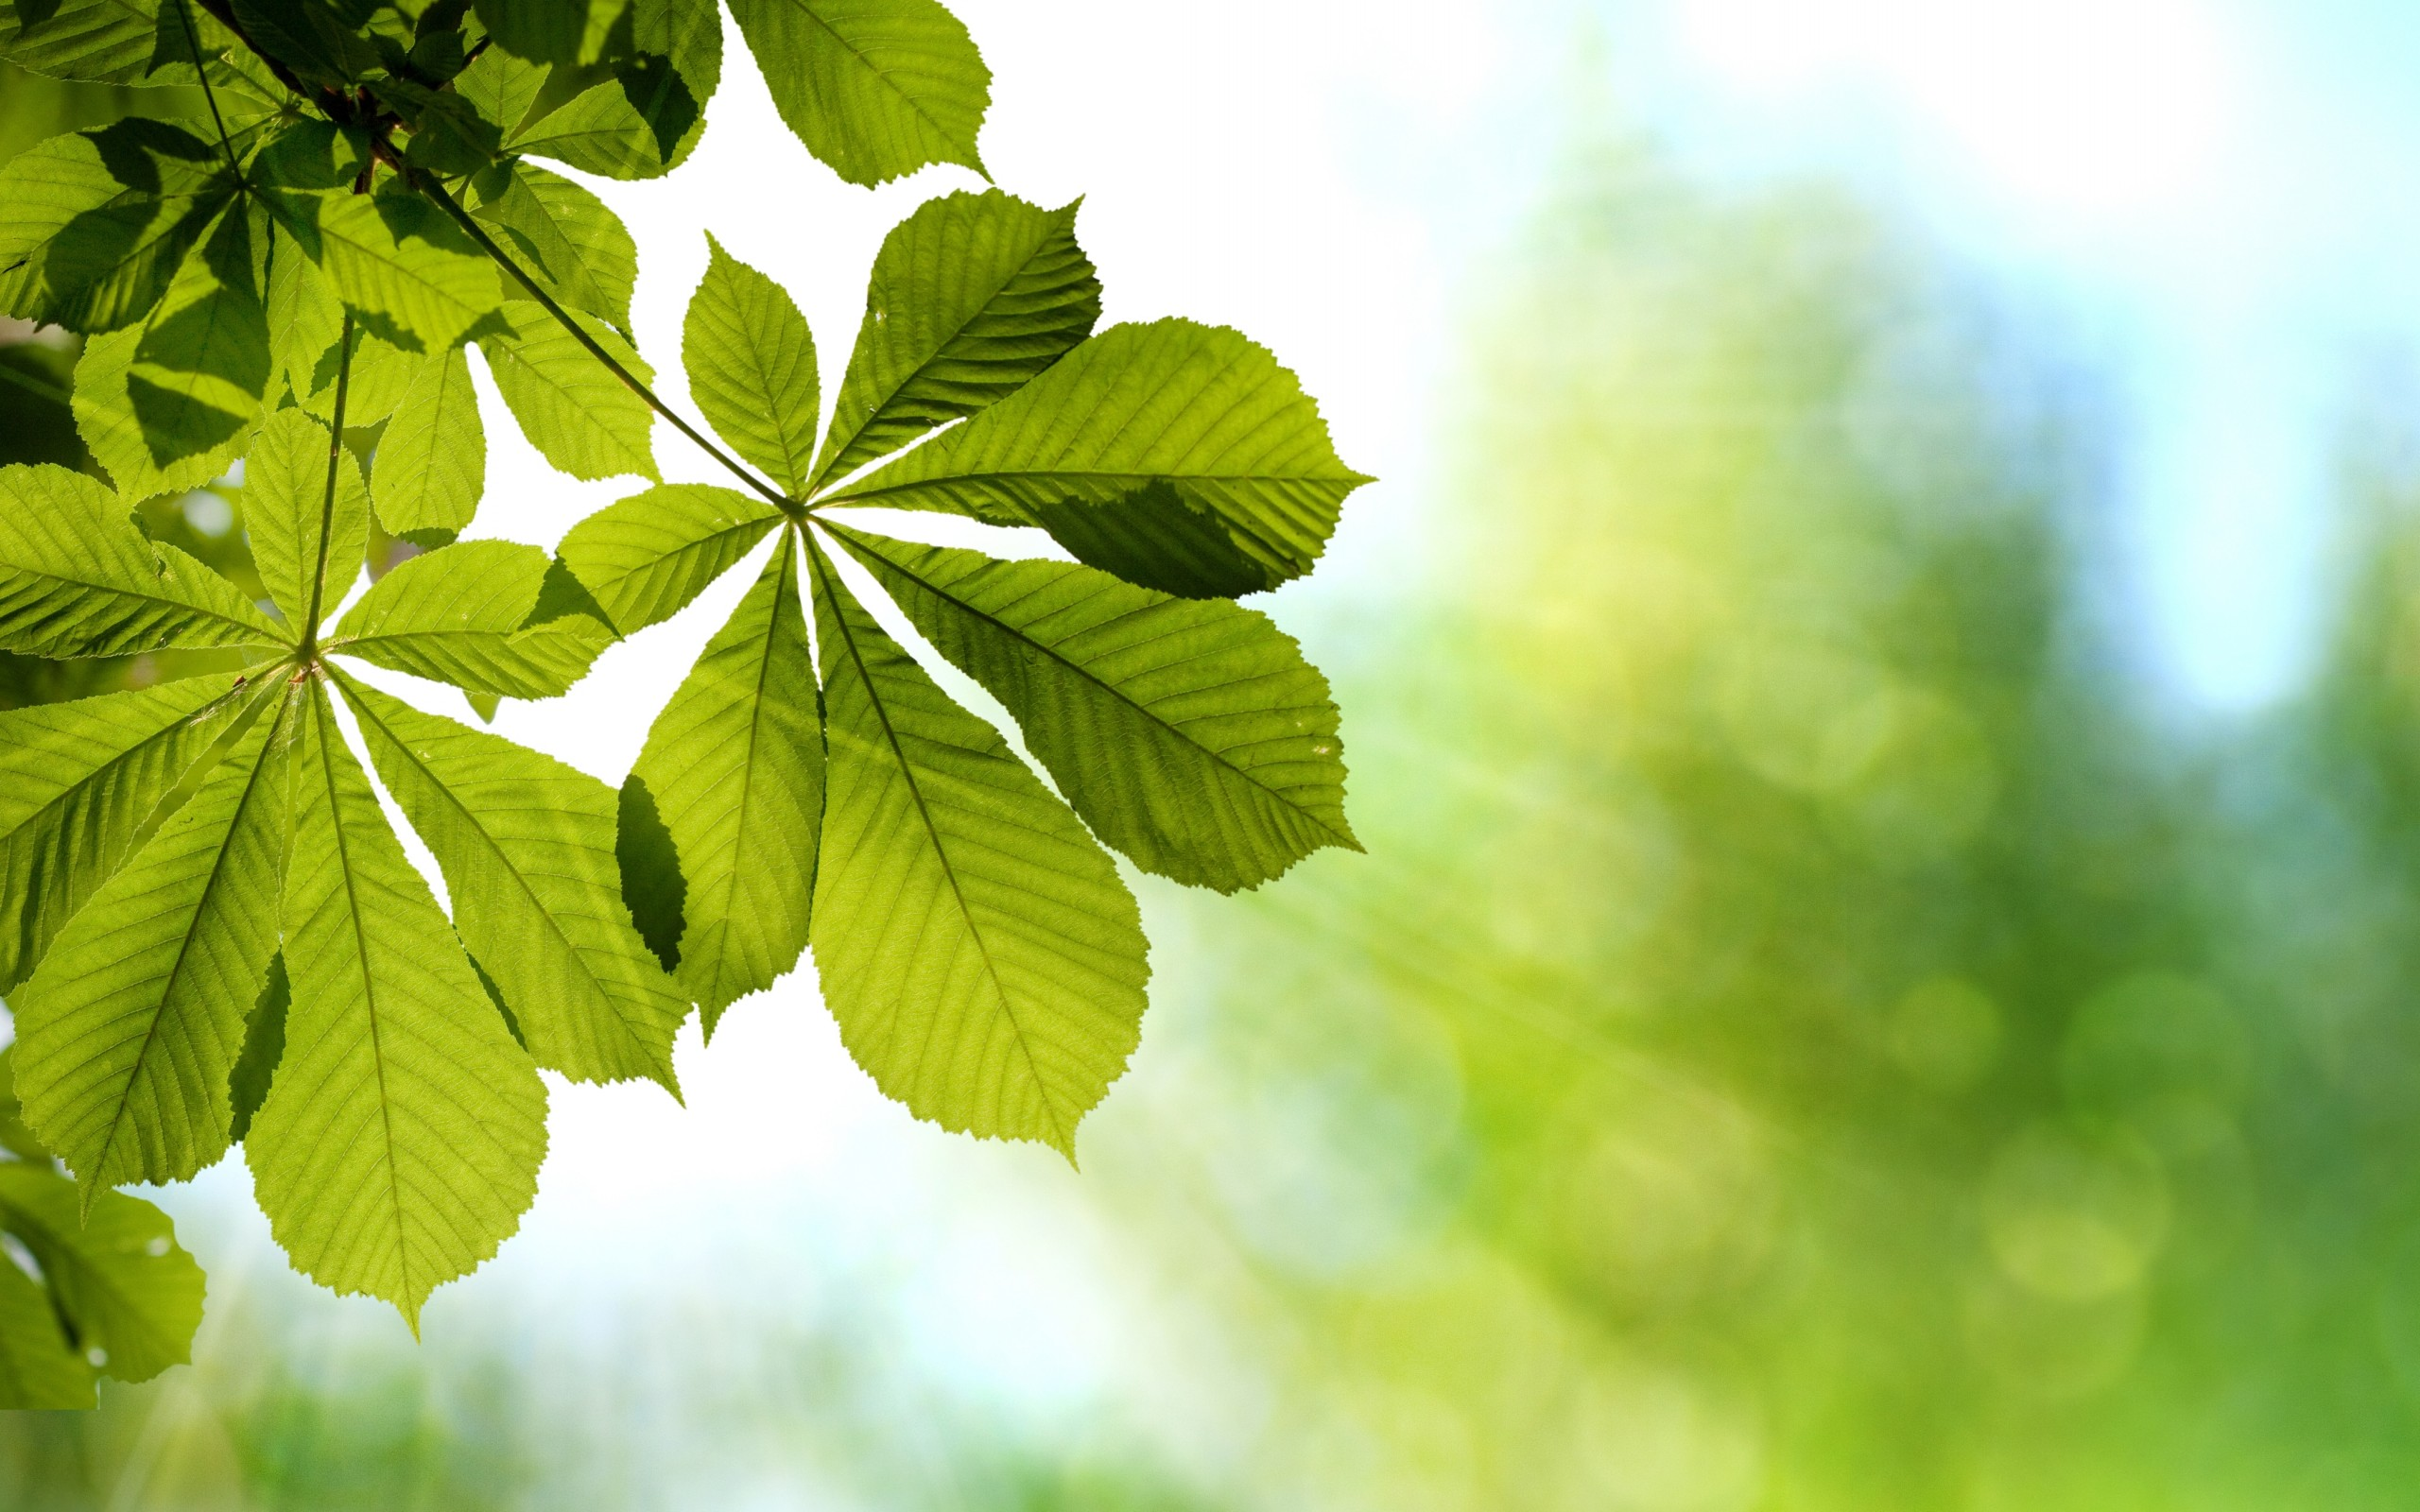
\includegraphics[scale=.5,angle=-90,origin=c]{leafs_02}}; % Background image
	\node[anchor=north west,inner sep=0pt] at (0,0) {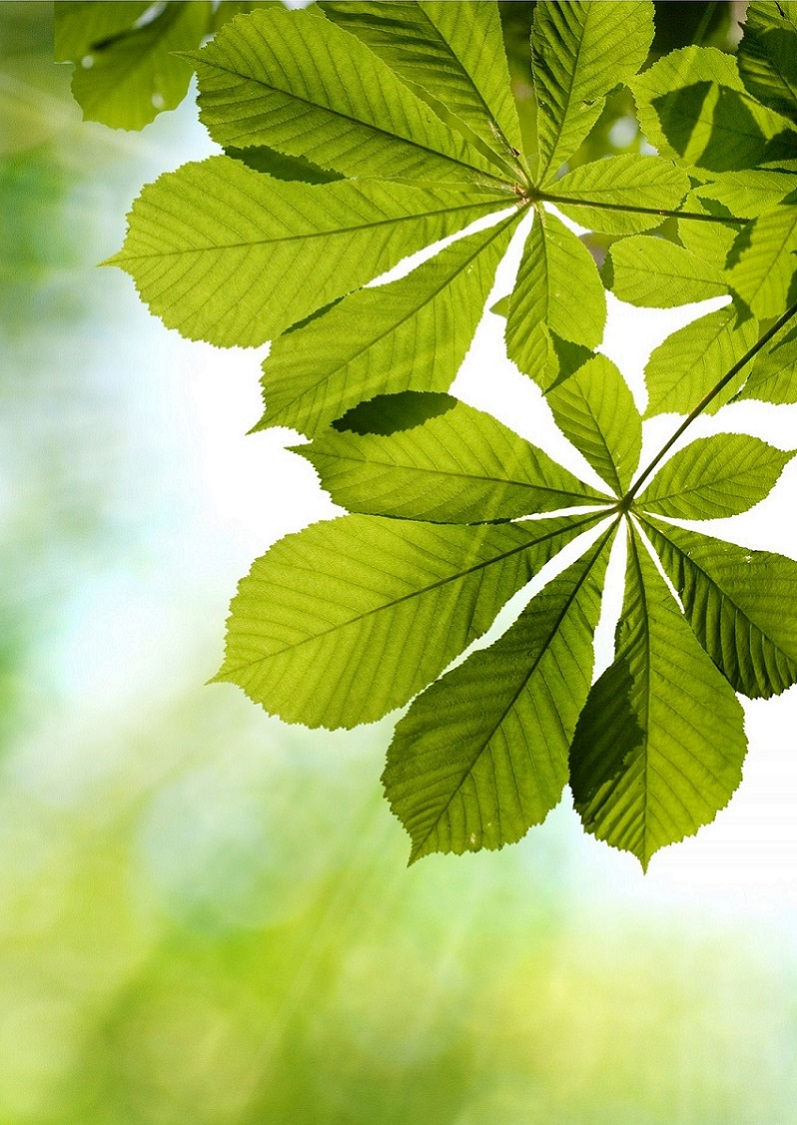
\includegraphics{leafs_04}}; % Background image
%	\draw[anchor=north] (midpoint) node [fill=ocre!30!white,fill opacity=0.6,text opacity=1,inner sep=1cm]{\Huge\centering\bfseries\sffamily\parbox[c][][t]{\paperwidth}{\centering SEMINÁRIOS PPG-EM / UERJ 2015\\[15pt] % Book title
%			{\huge PPG-EM UERJ 2015 SEMINARS}\\[20pt] % Subtitle
%			{\Large Programa de Pós-graduação em Engenharia Mecânica UERJ}
%		}}; % Author name
		\end{tikzpicture}};
\end{tikzpicture}
\vfill
\endgroup

\end{document}
